\documentclass[bachelor, och, book]{SCWorks}
\usepackage[T2A]{fontenc}
\usepackage[utf8]{inputenc}
\usepackage{graphicx}
\usepackage[sort,compress]{cite}
\usepackage{amsmath}
\usepackage{amssymb}
\usepackage{amsthm}
\usepackage{fancyvrb}
\usepackage{longtable}
\usepackage{array}
\usepackage[english,russian]{babel}
\usepackage{minted}
\usepackage{tempora}
\usepackage{titlesec}
\usepackage[colorlinks=false]{hyperref}
\usepackage{xcolor}
\usepackage{hyperref}

\definecolor{linkcolor}{HTML}{799B03} % цвет ссылок
\definecolor{urlcolor}{HTML}{799B03} % цвет гиперссылок

\hypersetup{pdfstartview=FitH,  linkcolor=linkcolor,urlcolor=urlcolor, colorlinks=true}

\hypersetup{ %содержание
colorlinks,
citecolor=black,
filecolor=black,
linkcolor=black,
urlcolor=black
}
\theoremstyle{remark}
\newtheorem{theorem}{Теорема}
\newtheorem{definition}{Определение}
\newtheorem{comment}{Замечание}

\begin{document}
    \hfill \break
    \hfill \break
    \hfill \break
    \hfill \break
    \hfill \break
    \hfill \break
    \hfill \break
    \hfill \break
    \hfill \break
    \hfill \break
    \hfill \break
    \hfill \break
    \begin{center}
        \Huge Лекции по Операционным системам
    \end{center}
    \hfill \break
    \hfill \break
    \hfill \break
    \hfill \break
    \hfill \break
    \hfill \break
    \hfill \break
    \hfill \break
    \hfill \break

    \begin{center} Сверстал: Кузякин Никита Александрович \end{center}
    \begin{center} По лекциям ИТМО \end{center}
    \begin{center}Плейлист с лекциями "--- \href{https://www.youtube.com/watch?v=NctMiqgVRxA&list=PLBWafxh1dFuyGGcWXmR_EngRkoUWvDFJi&index=1}{тут}\end{center}
    \thispagestyle{empty} % выключаем отображение номера для этой страницы
     
    \newpage
    \tableofcontents

    \part{Основы архитектуры ПК и операционных систем}
    \section{Архитектура компьютерных систем}

    Первоначальными двумя архитектурами компьютерных систем являются Гарвардская и Неймановская архитектуры.

    \begin{figure}[H]
        \begin{center}
            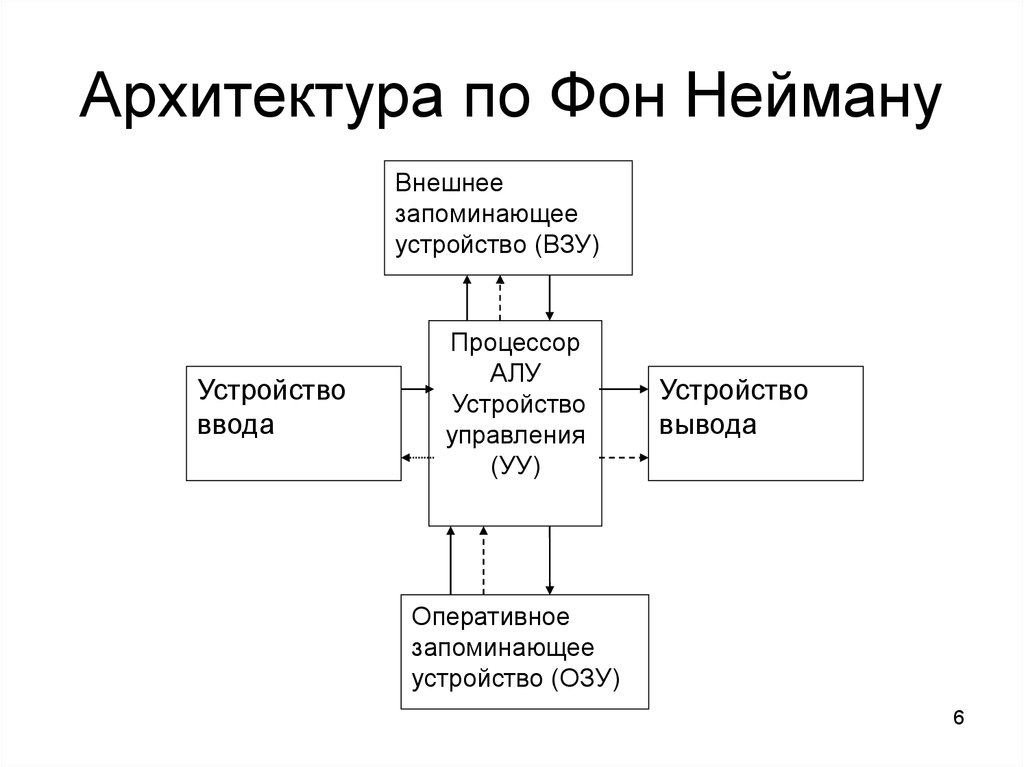
\includegraphics[scale=0.7]{res/Neumann_architecture.png}
        \end{center}
    \end{figure}

    \begin{figure}[H]
        \begin{center}
            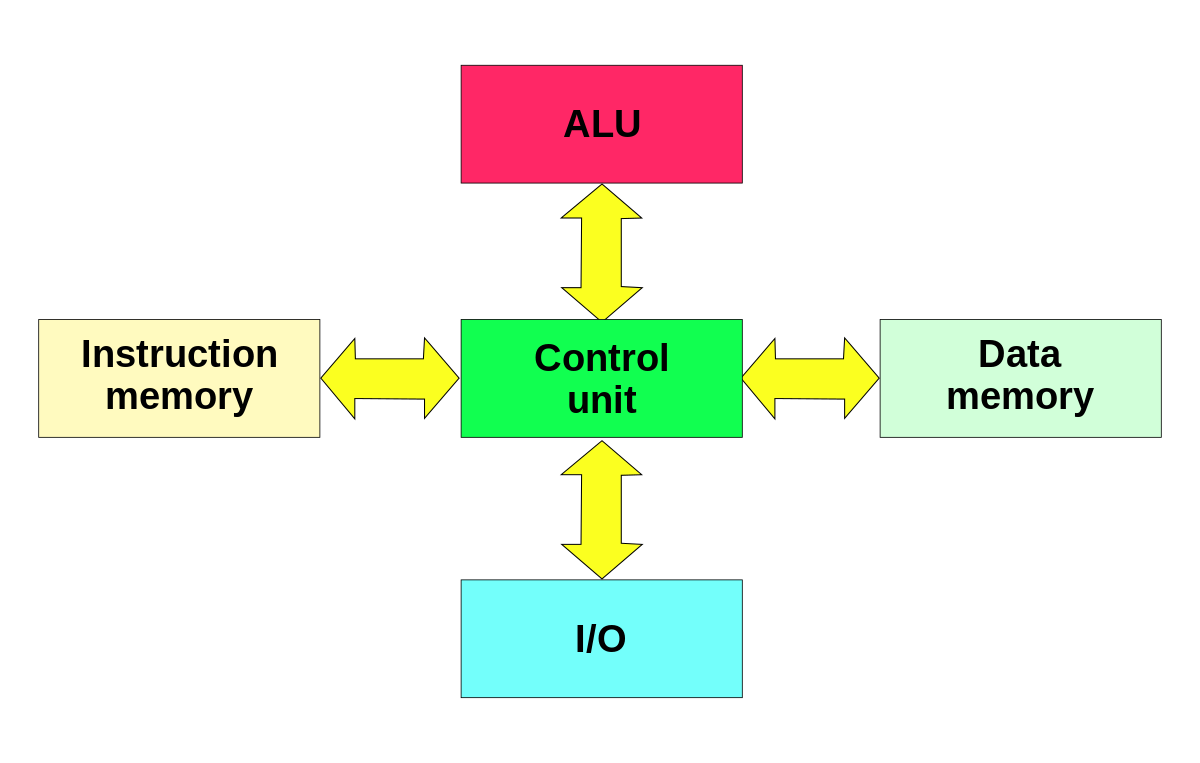
\includegraphics[scale=0.3]{res/Harvard_architecture.png}
            \caption{Гарвардская архитектура ЭВМ}
        \end{center}
    \end{figure}

    Любая вычислительная машины состоит из управляющего устройства (организует вычисления) и арифметико "= логического устройства (производит вычисление арифметических операций), а также различных видов памяти.
    
    В архитектуре фон Неймана предполагается, что есть единое управляющие устройство, память при этом общая (и данная, и программа в одно блоке).

    \textbf{Принципы архитектуры фон Неймана:} 

    \begin{itemize}[label=$\bullet$]
        \item Принцип однородности памяти "--- команды и данные хранятся в одной и той же памяти (внешне неразличимы).
        \item Принцип адресности "--- память состоит из пронумерованных ячеек, процессору доступна любая ячейка.
        \item Принцип программного управления "--- вычисления представлены в виде программы, состоящей из последовательности команд.
        \item Принцип двоичного кодирования "--- вся информация, как данные, так и команды, кодируются двоичными цифрами 0 и 1.
    \end{itemize}

    \hfill \break
    \begin{center}
        \textbf{UMA / NUMA}        
    \end{center}

    В архитектуре U\textbf{UMA} подразумевается, что все устройства являются одноранговыми. Те у любого устройства в системе равные права на доступ к памяти и системные характеристики обращения к ней. 

    \begin{figure}[H]
        \begin{center}
            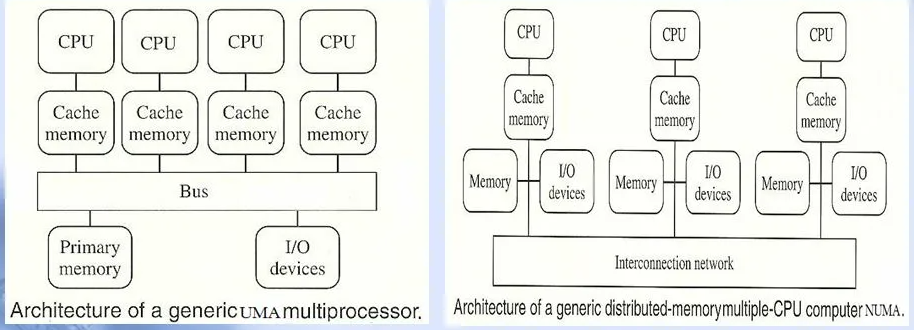
\includegraphics[scale=0.5]{res/UMA-NUMA_architecture.png}
            \caption{Гарвардская архитектура ЭВМ}
        \end{center}
    \end{figure}

    Минусом данной архитектуры является, то что тяжело организовать доступ к памяти для большого числа процессоров.

    В архитектуре \textbf{NUMA} у нас есть память, которая находится ближе к какому-то процессору и память, которая доступна через коммутатор (передает данные через порты). 

    Адресное пространство для данной архитектуры является общим.

    Огромным плюсом является, что можно заменять ее части прямо во время работы, что сильно повышает надежность системы.

    \section{Обзор элементов компьютерных систем}
    
    \subsection{Процессор}
    \begin{figure}[H]
        \begin{center}
            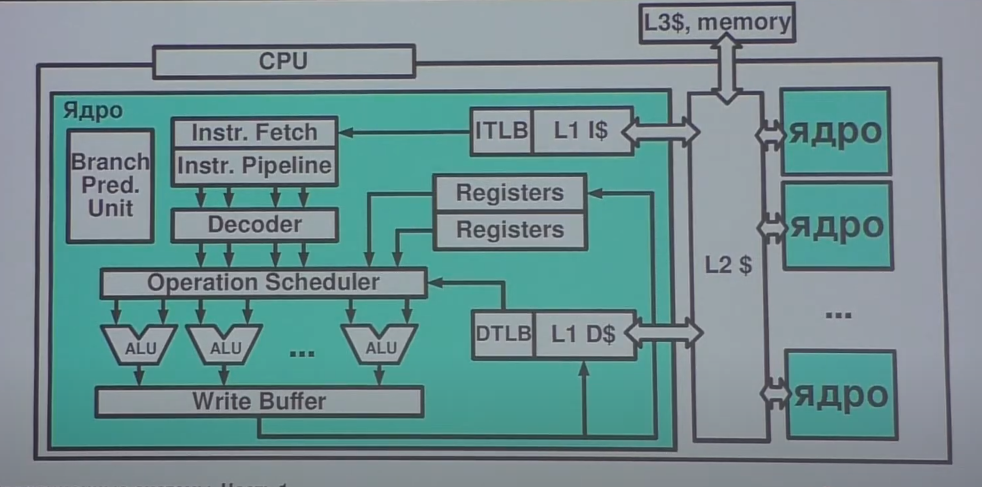
\includegraphics[scale=0.5]{res/processor.png}
        \end{center}
    \end{figure}

    Составляющие: 
    
    \begin{enumerate}
        \item Арифметико-логическое устройство (АЛУ), выполняющее действия над операндами.
        \item Буфер ассоциативной трансляции (TLB) "--- хранит информацию, есть ли такие"=то данные в данном кэше.
        \item Кэш процессора, используемый микропроцессором компьютера для уменьшения среднего времени доступа к компьютерной памяти. Делится на L1 i и L1 d. Один из них хранит набор инструкций для работы с кэшем, другой данные.
        \item Регистры для хранения данных, адресов и служебной информации.
        \item Декодер команд.
        \item Буфер для записи "--- хранит данные, пока буфер не освободится для записи.
        \item Branch Pred. Unit "--- предполагает куда будут записаны данные, по какому адресу (последовательно или с каким"=то отступом).
        \item Instr. Pipeline "--- это метод реализации параллелизма на уровне команд в пределах одного процессора.
    \end{enumerate}

    \hfill \break
    Важно помнить, что процессор выполняет команды последовательно. Пока один компонент выполняет одно действие, другой выполняет другое (они не останавливаются пока одни данные пройдут от начала до конца).

    \begin{definition}
        \textbf{Виртуальная память} "--- это подход к управлению памятью компьютером, который скрывает физическую память (в различных формах, таких как: оперативная память, ПЗУ или жесткие диски) за единым интерфейсом, позволяя создавать программы, которые работают с ними как с единым непрерывным массивом памяти с произвольным доступом.
    \end{definition}

    \begin{figure}[H]
        \begin{center}
            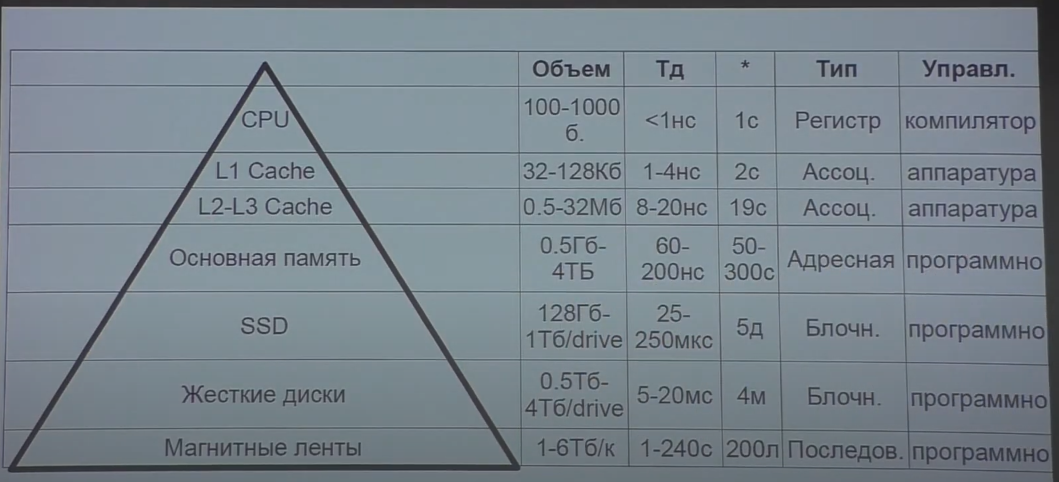
\includegraphics[scale=0.4]{res/memory-pyramid.png}
        \end{center}
    \end{figure}

    Управляется компилятором "--- означает, что именно компилятор определяет, как именно ваша программа будет взаимодействовать с данным блоком памяти, те что в какие регистры запишется и тд. 


    \section{Общие сведения об операционных системах}
    
    \subsection{Функции OS}
    
    \begin{itemize}[label=$\bullet$]
        \item Разработка программ.
        \item Выполнение программ.
        \item Доступ к устройствам ввода / вывода.
        \item Контролируемый доступ к файлам.
        \item Доступ к системе и системным ресурсам.
        \item Обнаружение и обработка ошибок.
        \item Учет пользования и диспетчеризация ресурсов.
        \item Предоставление ключевых интерфейсов (ISA "--- набор команд, ABI "--- бинарный интерфейс приложения, API "--- интерфейс прикладных программ).
    \end{itemize}
    
    \subsection{Оператор ЭВМ}
    Что должен делать оператор?
    \begin{enumerate}
        \item получить программу с данными от программиста.
        \item подготовить программу к загрузке.
        \item загрузить программу и компилятор.
        \item запустить программу на вычисление.
        \item распечатку с результатом передать программисту.
    \end{enumerate}

    Минусами оператора ЭВМ является: наличие расписания машинного времени и долгое время подготовки к работе.

    \subsection{Пакетная обработка}
    В следствие минусов оператора ЭВМ появилась пакетная обработка.

    Появился первый Системный монитор, который включал в себя: обработчик прерываний, драйверы устройств, планировщик заданий, интерпретатор командного языка и было отведено пространство под пользовательские программы и данные.


    \subsection{Многозадачность}

    Одним из главных минусов первых ЭВМ было то, что вовремя вывода, ввода или работы других устройств процессор простаивал. В следствие этого появилась концепция многозадачности.

    \begin{figure}[H]
        \begin{center}
            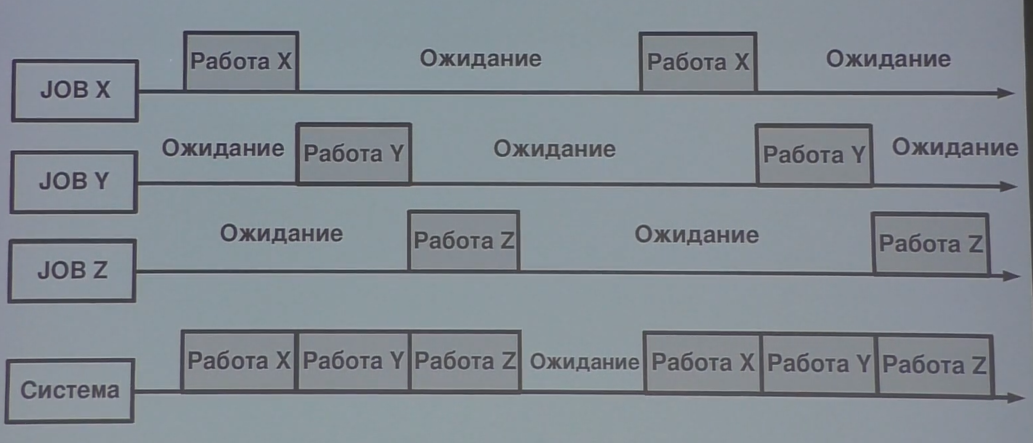
\includegraphics[scale=0.4]{res/multitasking.png}
            \caption{Схема многозадачности первых ЭВМ}
        \end{center}
    \end{figure}
    
    \subsection{Разделение времени}
    
    Следующим нововведением в ЭВМ стало исключение оператора и добавление пользователей. Каждому пользователю выдавалось часть времени процессора с использованием квантового времени. В следствие этого появились проблемы разделения ресурсов и защита одних программ от других.

    \section{Основные задачи OS}

    \subsection{Управление процессами}

    \begin{definition}
        \textbf{Процесс} (с точки зрения обывателя) "--- экземпляр программы во время ее исполнения.
    \end{definition}
    
    \begin{definition}
        \textbf{Процесс} (с точки зрения OS) "--- единица потребления ресурсов OS, в которой существует последовательность действий, текущее состояние и набор связанных ресурсов.
    \end{definition}
    
    \begin{figure}[H]
        \begin{center}
            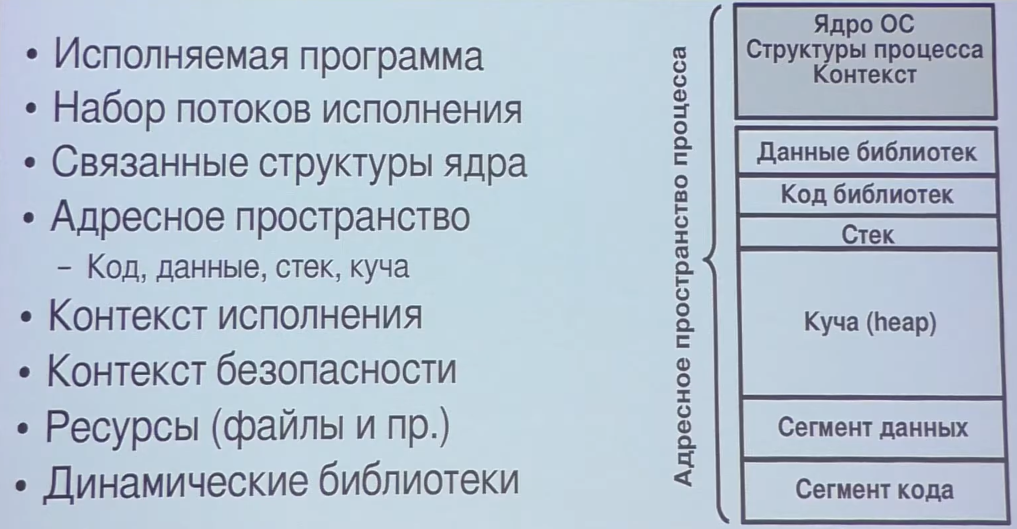
\includegraphics[scale=0.4]{res/process-structure.png}
            \caption{Структура процесса}
        \end{center}
    \end{figure}

    Для того, чтобы создать процесс, необходимо создать все части адресного пространства представленного на рисунке 4.

    Процесс создается не так быстро, поэтому для вычислений на процессоре можно просто создать поток (по сути он будет представлять набор регистров) и с помощью него провести вычисления. Это все и является контекстом.

    Когда создается процесс, ядро OS должно построить для ресурсов, которое он будет потреблять систему (описание ресурсов) (в линуксе task structure). 

    Проблемы современных процессов:

    \begin{itemize}[label=$\bullet$]
        \item Защита памяти процессов "--- недетерминированное поведение процесса, к примеру обращение не к своей памяти, может нарушить другие процессы.
        \item Взаимные блокировки "--- есть два процесса, один из них захватил один ресурс, другой другой, и они пытаются также добавить к себе захваченный другим процессом ресурс. (deadlock, livelock, starvation)
        \item Проблема синхронизации "--- тк у нас может быть несколько процессов, а адресное пространство для них одно.
        \item Взаимное исключение доступа ресурсов.
    \end{itemize}

    \subsection{Виртуальная память}
    Для решения проблемы с единым адресным пространством была придумана виртуальная память.

    Управление памятью: 
    \begin{itemize}[label=$\bullet$]
        \item Изоляция процессов.
        \item Управление выделением и освобождением памяти (аллокаторы и мепинг памяти).
        \item Поддержка модулей (модульности) "--- динамическая загрузка и выгрузка модулей.
        \item Защита и контроль доступа "--- права на сегменты памяти.
        \item Долговременное хранение "--- запись информации на диск.
        \item Страничный обмен. 
    \end{itemize}

    \begin{definition}
        \textbf{Виртуальная память} "--- отдельное виртуальное адресное пространство для каждого процесса и ядра.
    \end{definition}

    Также виртуальная память подразумевает, что некоторые страницы нельзя выгружать из памяти, к примеру если они используются в большом количестве процессов.
    
    \subsection{Безопасность}
    Также важный аспект OS это то, на сколько она безопасна, на сколько она обеспечивает безопасность данных.

    Самым важным аспектом безопасности является протокол работы с информацией.

    Что должна обеспечивать OS:

    \begin{enumerate}
        \item Безопасность доступа к системе "--- защита от несанкционированного доступа.
        \item Конфиденциальность "--- невозможность неавторизованного доступа к данным.
        \item Целостность данных "--- защита данных от неавторизованного и нецелостного изменения.
        \item Аутентификация и авторизация.
    \end{enumerate}

    \subsection{Диспетчеризация и планирование ресурсов}

    Что важно учесть при планирование ресурсов (с точки зрения OS):

    \begin{itemize}[label=$\bullet$]
        \item Равноправие "--- пользователи, процессы и тд должны получать ресурсы равноправно. (Интересный факт: в UNIX приоритет процесса развернутого окна на 15 пунктов выше других).
        \item Дифференциация отклика "--- в некоторых задачах нужно понизить время отклика, к примеру в задачах выполняющихся в реальном времени.
        \item Общесистемная эффективность.
        \item Планировщик процессов, дисков и тд.
    \end{itemize}


    \section{Современные архитектурные концепции OS}

    \subsection{Архитектура ядер}

    \begin{figure}[H]
        \begin{center}
            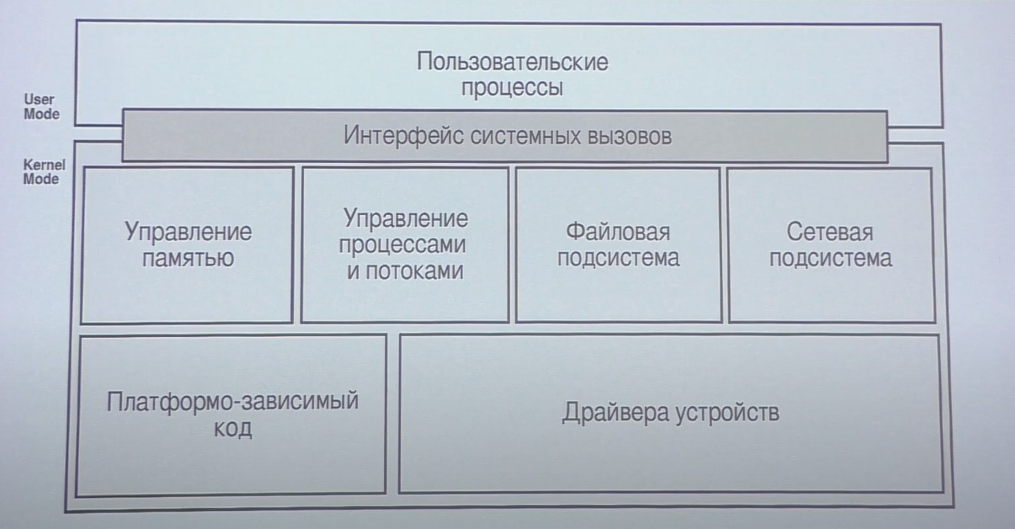
\includegraphics[scale=0.4]{res/OS-kernel-diagram.png}
            \caption{Схема ядра OS}
        \end{center}
    \end{figure}

    Управление памятью, процессами и потоками, файловая подсистема и сетевая подсистема работают на основе драйверов и платформо "= зависимого кода.

    \begin{figure}[H]
        \begin{center}
            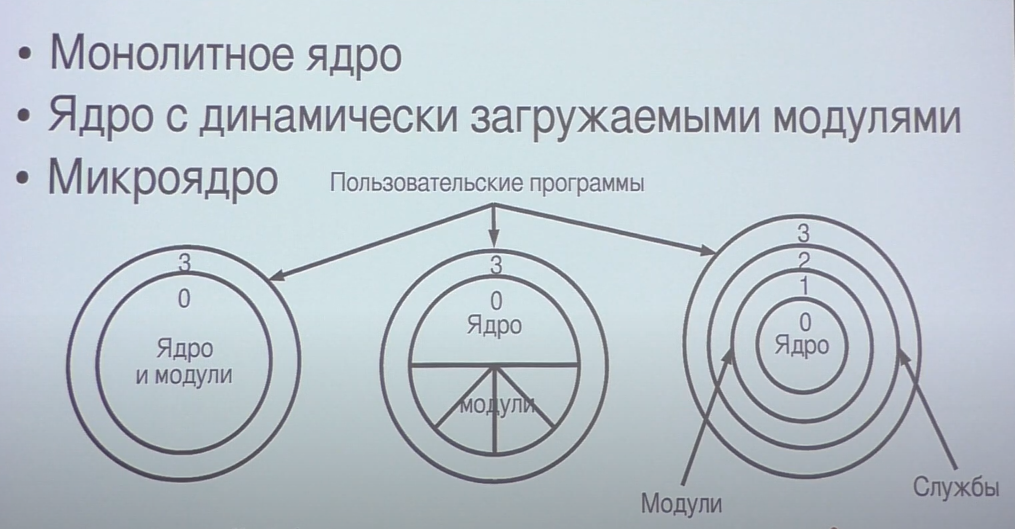
\includegraphics[scale=0.4]{res/kernel-architectures.png}
            \caption{Виды архитектур ядер OS}
        \end{center}
    \end{figure}

    Монолитное ядро "--- подразумевает, что для изменение чего"=то в ядре придется перекомпилировать OS. Подходит для систем где набор устройств определен и не будет изменяться. 0 уровень "--- ядро и встроенные в него модули, 3 уровень "--- пользовательские программы. 1 и 2 не используются.

    Ядро с динамически загружаемыми модулями имеет возможность загрузить модули во время выполнения операционной системы.
    
    Микроядро "--- концепция, в которой само ядро занимается базовыми задачами: диспетчеризация процессов и выделение памяти. 1 и 2 уровни занимают остальные задачи, реализованные в виде сервисов. Пользовательские приложения работают на 3 уровне. Из"=за частого переключения контекстов это работает очень медленно. 

    \subsection{Многопоточность}
    Из"=за сложности создания процесса была придумана концепция реализации внутри процесса потоков. Tread "--- нить / поток.

    Библиотека порождающая потоки на UNIX системах Posix Treads.
    
    Существует множество концепций реализации потоков, они будут рассмотрены в следующих параграфах.

    \subsection{SMP и ASMP}
    
    \textbf{Symmetric multiprocessing} "--- процессы равны, процесс выполняется на нескольких процессорах одновременно. Это дает следующие плюсы: простота разработки и производительность, более высокая надежность (при отказе выполнить процесс, его могут выполнить другие), масштабируемость приложений, динамическое добавление ресурсов процессора. 

    \textbf{Asymmetric multiprocessing} "--- в системе с асимметричной многопроцессорностью не все процессоры играют одинаковую роль. Например, система может использовать (либо на аппаратном, либо на уровне операционной системы) только один процессор для выполнения кода операционной системы, или поручать только одному процессору выполнение операций ввода-вывода. В других AMP-системах все процессоры могут выполнять код операционной системы и операции ввода-вывода, так что с этой стороны они ведут себя как симметричная многопроцессорная система, но определенная периферийная аппаратура может быть подсоединена только к одному процессору, так что со стороны работы с этой аппаратурой система предстаёт асимметричной. Более дешевая альтернатива в системах, которые поддерживали SMP.
 
    \textbf{Многопоточность $!=$ Многопроцессорность}

    \subsection{Виртуализация}

    \textbf{Виртуальные машины (интерпретаторы)} "--- по сути программы, которые работают под выполнением другой программы. Как примеры: JS в браузере, python, JAVA VM. Это позволяет поднять уровень абстракции.

    \begin{definition}
        \textbf{Интерпретация} — построчный анализ, обработка и выполнение исходного кода программы или запроса, в отличие от компиляции, где весь текст программы, перед запуском анализируется и транслируется в машинный или байт-код без её выполнения.
    \end{definition}

    \textbf{Контейнеры приложений} "--- позволяет писать приложения один раз и запускать их где угодно. Разработчики могут создавать и развертывать приложения быстрее и безопаснее, чем при традиционном подходе к написанию кода — когда он разрабатывается в определенной вычислительной среде, а его перенос в новое место, например из тестовой среды в продуктивную, часто приводит к ошибкам выполнения кода.

    \begin{definition}
        \textbf{Контейнер приложения} "--- экземпляр исполняемого программного обеспечения (ПО), который объединяет двоичный код приложения вместе со всеми связанными файлами конфигурации, библиотеками, зависимостями и средой выполнения.
    \end{definition}

    Смысл и главное преимущество технологии в том, что контейнер абстрагирует приложение от операционной системы хоста, то есть остается автономным, благодаря чему становится легко переносимым — способным работать на любой платформе.

    Примеры: Docker, Solaris containers, Linux containers. 

    \textbf{Аппаратурная виртуализация} "--- виртуализация с поддержкой специальной процессорной архитектуры. В отличие от программной виртуализации с помощью данной техники возможно использование изолированных "гостевых" операционных систем.

    Примеры: Virtual BOX, KVM.


    \textbf{Облачные технологии} "--- по сути облачная виртуализация, главным плюсом является, что в случае сбоя одной физической системы, данные иммигрируют на другую систему и продолжат выполняться. Данные технологии построены на базе аппаратурной виртуализации.

    \section{Основные понятия надежности операционной системы}

    \subsection{Надежность и отказоустойчивость}

    \textbf{Отказоустойчивость} "--- способность системы продолжать работу при аппаратных или програмных ошибках.

    Для обеспечения отказоустойчивости нужно:

    \begin{itemize}[label=$\bullet$]
        \item Избыточность аппаратуры(двойное, тройное резервирование).
        \item Аппаратная "горячая" замена компонентов.
        \item Программная поддержка OS выведения компонентов из системы и их подключения.
        \item Организация уровней хранения RAID в дисковой подсистеме.
    \end{itemize}

    \textbf{Надежность} "--- вероятность бесперебойной работы системы до времени t, при условие ее корректной работы в t = 0.

    Среднее время наработки на отказ MTTF = $\int_{0}^{x} R(t) \ d t$, включает в себя время на перезагрузку, ремонта или замены неисправного компонента, установки (переустановки) OS или ПО.

    Коэффициент доступности "--- процент времени, когда система или служба доступна для запросов пользователей.

    Простой (downtime) "--- время, в течение которого система недоступна

    Безотказная работа "--- когда система находится в продуктивной работе.

    \subsection{Сбои}

    \hfill \break
    Какие бывают отказы:
    \begin{itemize}[label=$\bullet$]
        \item Ошибочное состояние аппаратуры или ПО в результате сбоя компонентов.
        \item Ошибки оператора.
        \item Физические помехи окружающей среды.
        \item Ошибки проектирования, программирования, структуры данных и тд.
        \item Могут быть: постоянные, временные (однократные или переодические).
    \end{itemize}

    \hfill \break
    Методы резервирования: 
    \begin{itemize}[label=$\bullet$]
        \item Физическая избыточность (компонентов, серверов). 
        \item Временная избыточность (повтор вычислений).
        \item Информационная избыточность (ECC, RAID).
    \end{itemize}

    \hfill \break
    Методы повышения отказоустойчивости:

    \begin{itemize}[label=$\bullet$]
        \item Изоляция процессов 
        \item Разрешение блокировок при прараллелизме
        \item Виртуализация
        \item Точки восстановления и откаты
    \end{itemize}

    \section{Общая архитектура UNIX / Linux}
    В UNIX появилась ключевая концепция: все есть файл или процесс. Также появился принцип: одна программа "--- одна функция. Также использовалась концепция минимизации ядра, реализация на C и унификация файлов. 

    \textbf{SINGL UNIX Specification} "--- общее название для семейства стандартов, которым должна удовлетворять операционная система, чтобы называться "UNIX".

    \textbf{UNIX системы} "--- AIX, MAC OS X, Solaris.

    \textbf{UNIX like системы} "--- Linux, Free BSD, Open Solaris.

    \textbf{Подробно архитектуру ядра Linux можно посмотреть по ссылке}: 
    
    \href{https://makelinux.github.io/kernel/map/}{https://makelinux.github.io/kernel/map/}

    \hfill \break
    Основные подсистемы Linux:
    \begin{itemize}[label=$\bullet$]
        \item Процессы и планировщик задач "--- создает, управляет и планирует процессы. 
        \item Виртуальная память "--- выделяет виртуальную память для процессов и управляет ею.
        \item Физическая память "--- управляет пулом кадров страниц и выделяет страницы для виртуальной памяти.
        \item Файловая система "--- представляет глобальное иерархическое пространство имен для файлов и функции для работы с файлами.
        \item Драйверы символьных устройств "--- управление устройствами, которые требуют от ядра отправки и получения данных по одному байту.
        \item Драйверы блочных устройств "--- управление устройствами, которые читают и записывают данные блоками. 
        \item Сетевые протоколы (TCP/IP)"--- поддержка пользовательского интерфейса сокетов для набора протоколов.
        \item Драйверы сетевых устройств.
        \item Ловушки и отказы "--- обработка генерируемых прерываний.
        \item Прерывания "--- обработка прерываний от периферийных устройств. 
        \item Сигналы и IPC "--- управление межпроцессорным взаимодействием.
    \end{itemize}


    \section{Общая архитектура Windows}
    
    В первых версиях Windows была надстройкой над операционной системой DOS. В данный момент у Windows есть несколько линеек: для мобильных устройств, для ПК и серверная.

    \begin{figure}[H]
        \begin{center}
            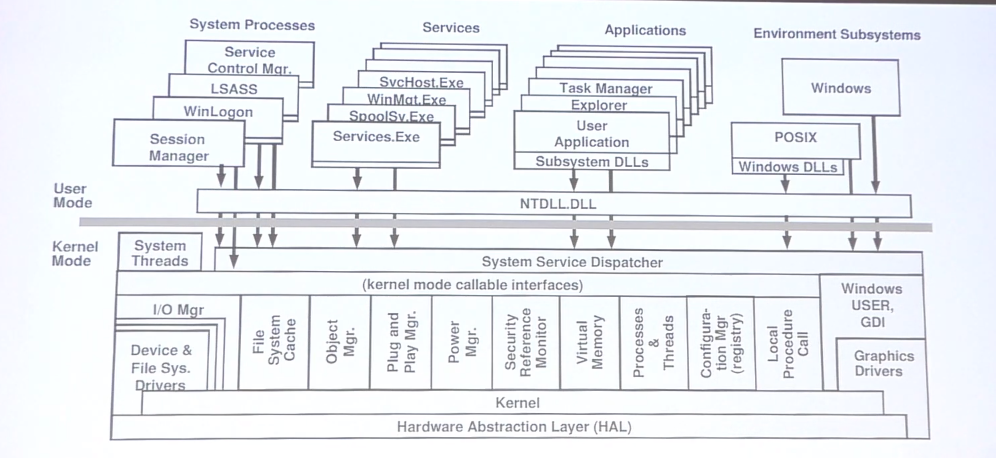
\includegraphics[scale=0.5]{res/Windows-architecture.png}
            \caption{Архитектура Windows}
        \end{center}
    \end{figure}

    Как не странно архитектура Windows очень похожа на архитектуру UNIX.

    Интерфейс системных вызовов "--- NTDLL.dll

    Также подсистемы Windows похожи на подсистемы в Linux.

    Plag and play Mgr. "--- система позволяющая легко ставить драйверы, без указания портов и тд.
    
    Одним из отличий является графический интерфейс интегрированный в ядро.

    \textbf{WinAPI} "--- это библиотеки динамической компоновки (DLL), которые являются частью Windows операционной системы. Они используются для выполнения задач, когда сложно написать эквивалентные процедуры. Например, Windows предоставляет функцию с именем FlashWindowEx, которая позволяет сделать заголовок строки приложения чередующимся между светлыми и темными оттенками. Позволяет легко написать приложение, которое будет совместимо с любой версией Windows.

    \begin{figure}[H]
        \begin{center}
            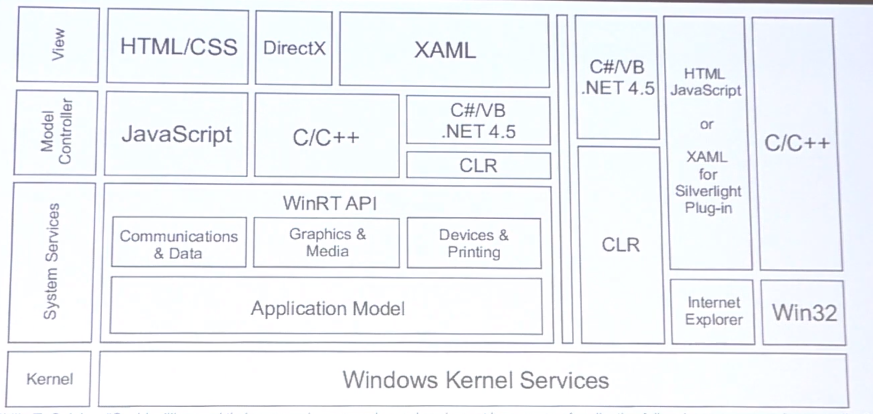
\includegraphics[scale=0.5]{res/WinAPI.png}
            \caption{Схема WinAPI}
        \end{center}
    \end{figure}

    Другие важные компоненты Windows:
    \begin{itemize}[label=$\bullet$]
        \item Гипервизор Hyper"=V "--- запуск гостевых операционных систем.
        \item Firmware "--- содержимое энергонезависимой памяти любого цифрового вычислительного устройства — микрокалькулятора, сотового телефона, GPS-навигатора и т. д., в которой содержится его программа.
        \item  Terminal Servers.
        \item Объекты "--- все вещи в системе сделаны в виде объектов.
        \item Реестр.
        \item Оснастки "--- специальная вспомогательная программа для администрирования выделенного пула задач.
    \end{itemize}

    \section{Средства для отладки Linux}
    \subsection{Стандартные средства}
    \begin{figure}[H]
        \begin{center}
            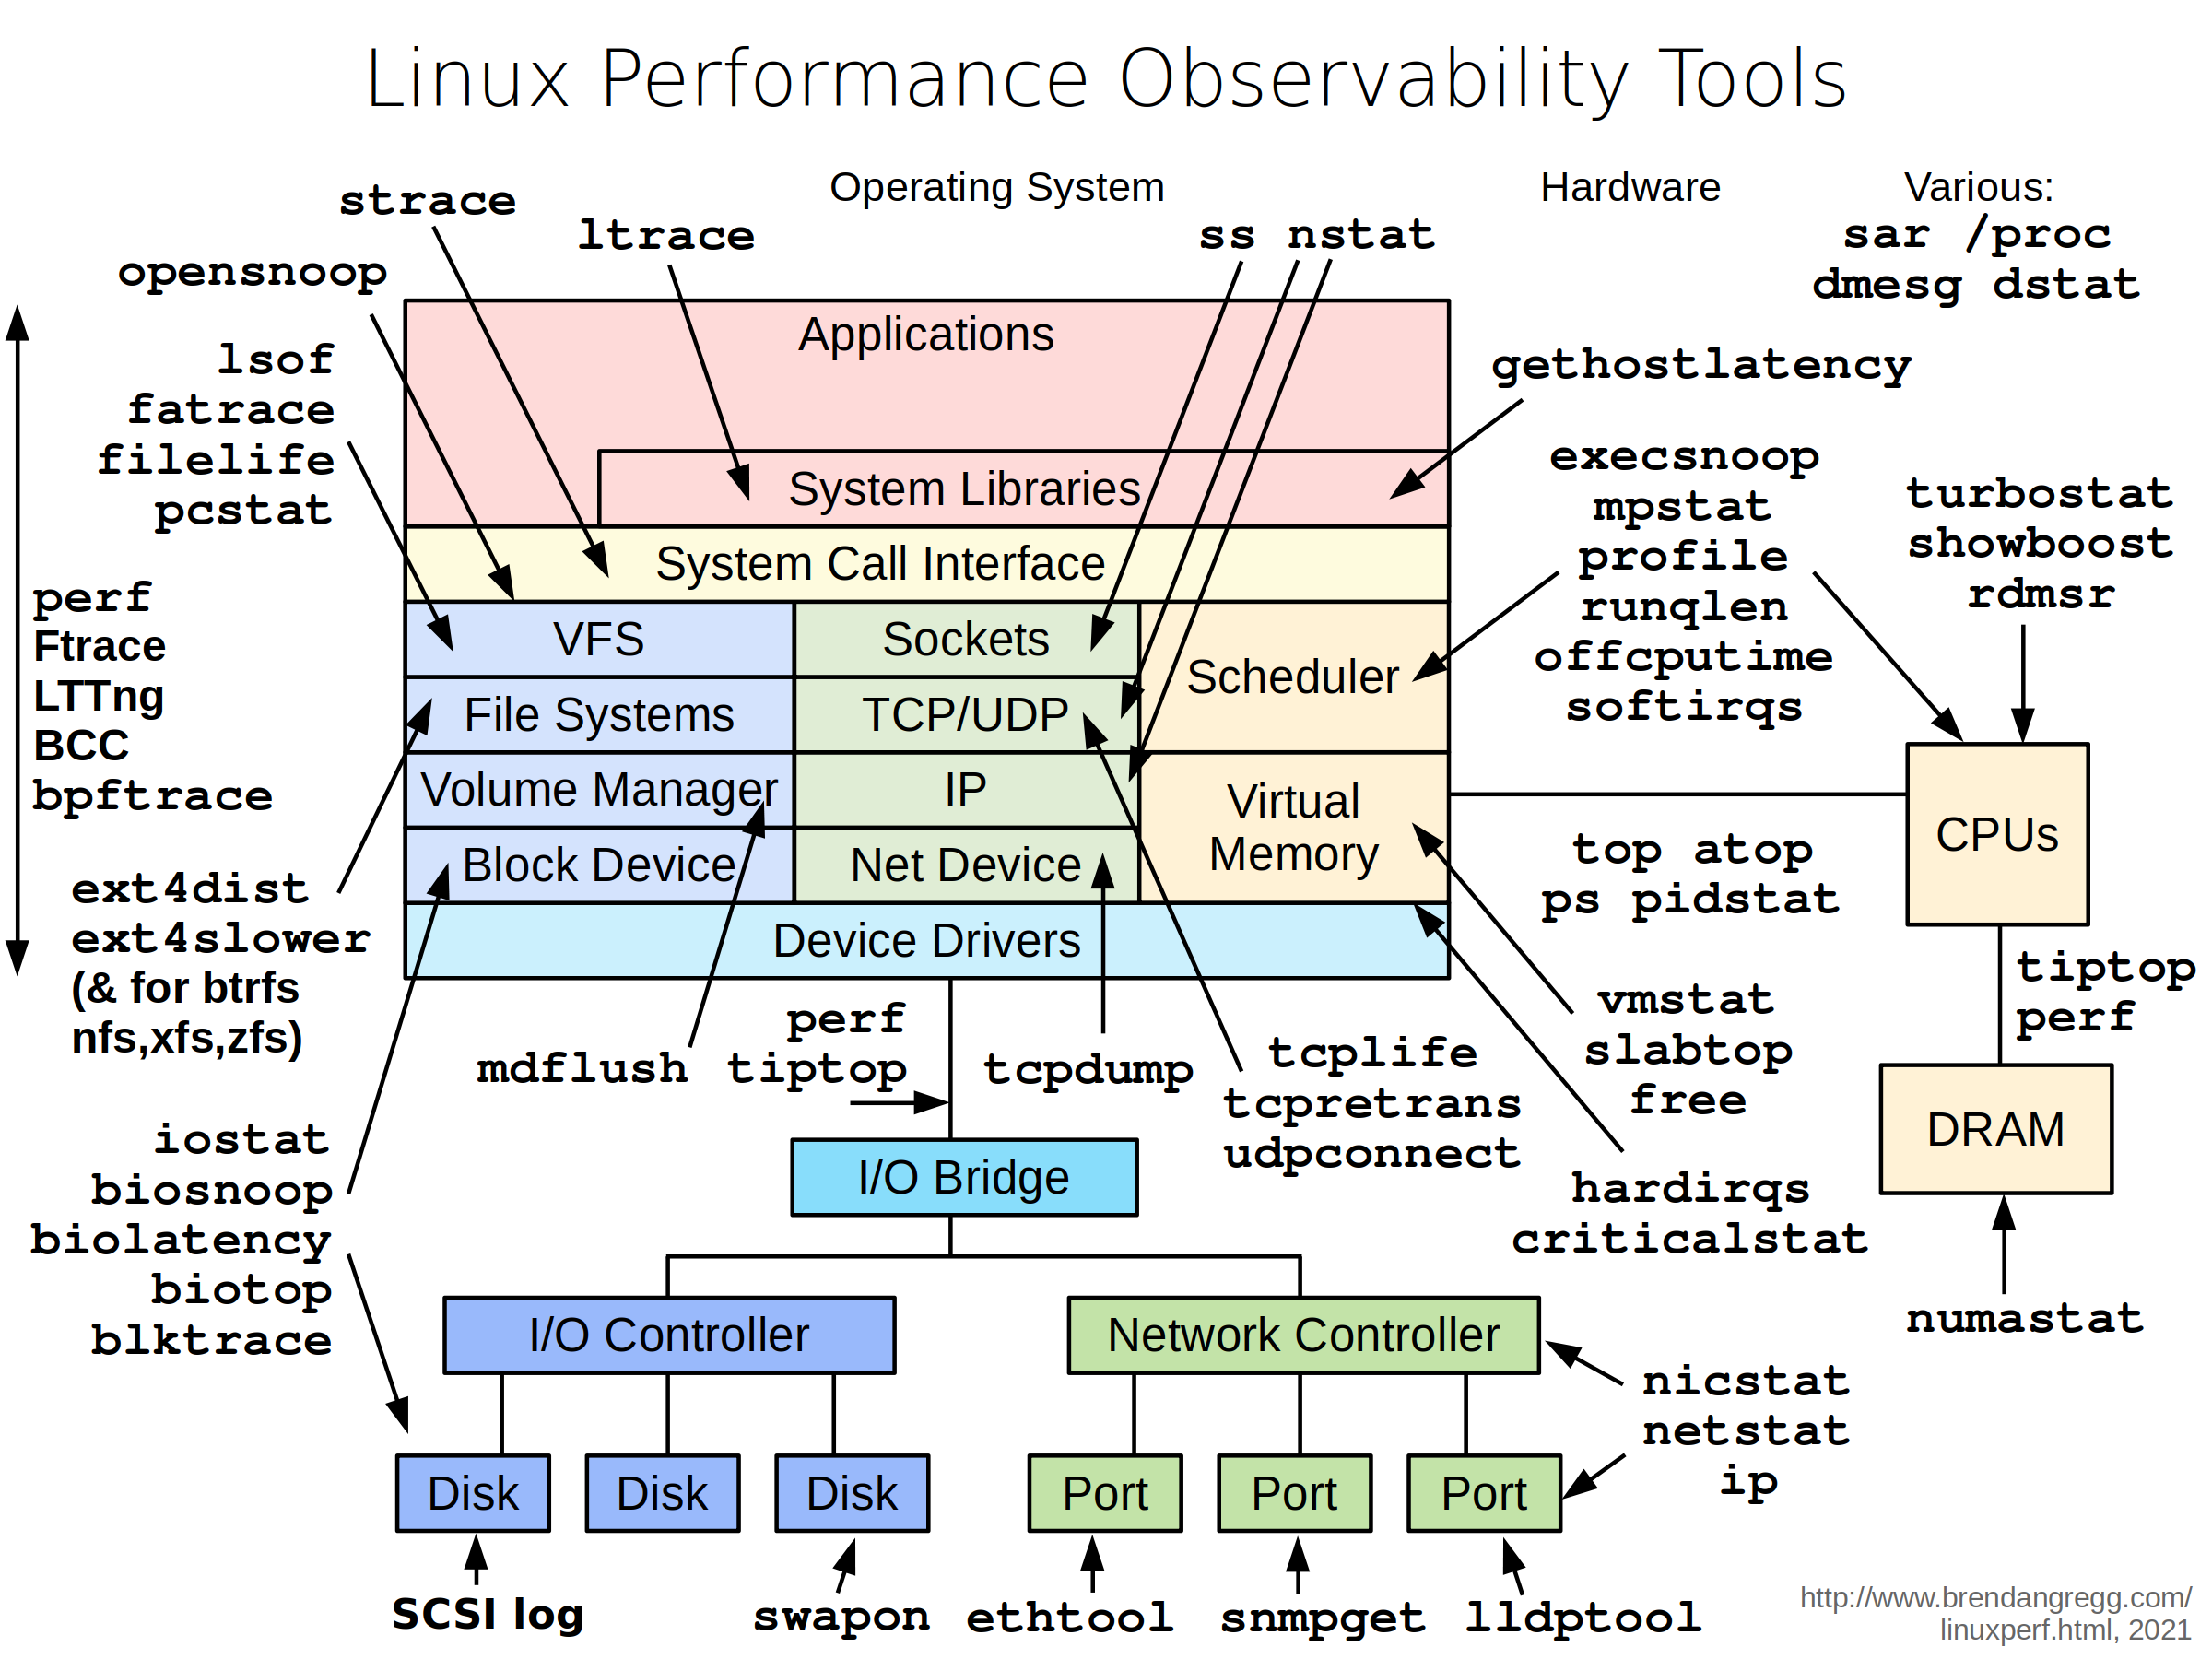
\includegraphics[scale=0.2]{res/linux-observability-tools.png}
            \caption{Утилиты для отладки линукс}
        \end{center}
    \end{figure}

    Ядро операционной системы накапливает большове количество различных счетчиков. И все представленные на рисунке 9 утилиты, по сути просто дают доступ к этим счетчикам, те никаких доп вычислений не производится.


    \begin{center}
        \textbf{Стандартные средства наблюдения за счетчиками}
    \end{center}

    \textbf{sar} "--- утилита, которая позволяет посмотреть информацию о счетчиках любой подсистемы Linux. 

    Подробно ознакомиться можно здесь:  \href{https://greendail.ru/node/monitoring-proizvoditelnosti-linux-na-primere-sar}{https://greendail.ru/node/monitoring-proizvoditelnosti-linux-na-primere-sar}

    \begin{figure}[H]
        \begin{center}
            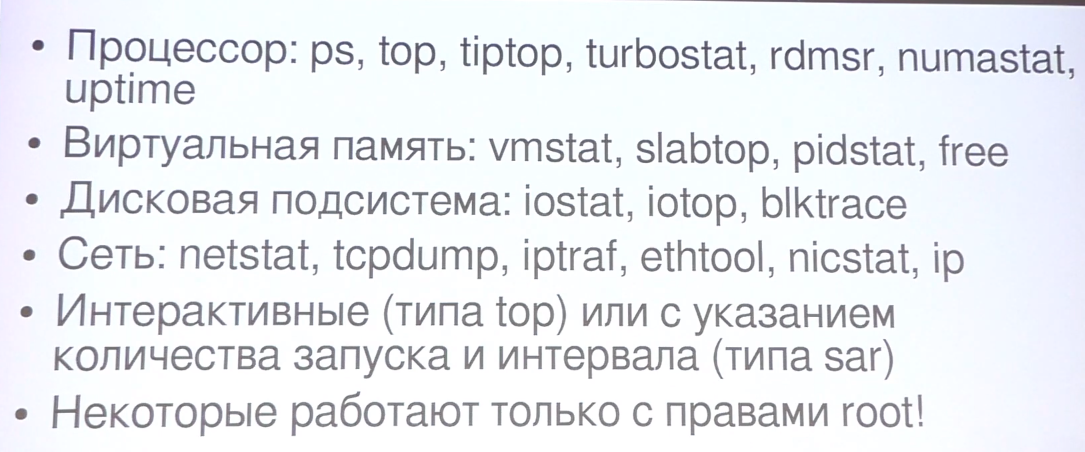
\includegraphics[scale=0.45]{res/standart-debug-ytil-linux.png}
            \caption{Другие встроенные утилиты}
        \end{center}
    \end{figure}


    Утилиты обычно двух типов: интерактивные (можно изменять параметры системы) и статичные (просто предоставляют информацию).

    \subsection{/proc}

    \textbf{/proc} "--- виртуальная файловая система, которая содержащая файлы статистики и управляющая модулями ядра. По сути вся информация представлена в виде файловой системы. К примеру, информация о процессоре будет лежать в каталоге /proc/cpuinfo.

    \subsection{Трассировщики}

    \begin{itemize}[label=$\bullet$]
        \item Трассировка системных вызовов: strace
        \item Трассировка вызовов библиотек: ltrace
        \item Трассировка lock -ф: bpftrace
    \end{itemize}

    Также одно из средств отладки, с помощью которого легко увидеть логи системных вызовов.

    \subsection{perf}
    Профилировщики "--- собирает системную информацию, которую вы указали.

    Основное предназначение профилировщиков "--- это взять ваше готовое приложение и посмотреть, что находится в ядре во время его запуска.

    Суть в том, что perf может собрать весь стэк трейс запущенной программы. Естественно, запущенный perf будет вносить задержку в работу всей системы. Но у нас есть флаг -F \#, где \# ― частота сэмплирования, измеряемая в Гц.

    К примеру perf record df -h запишет данные любой команды Perf, которую вы хотите сохранить для использования в будущем.

    \begin{figure}[H]
        \begin{center}
            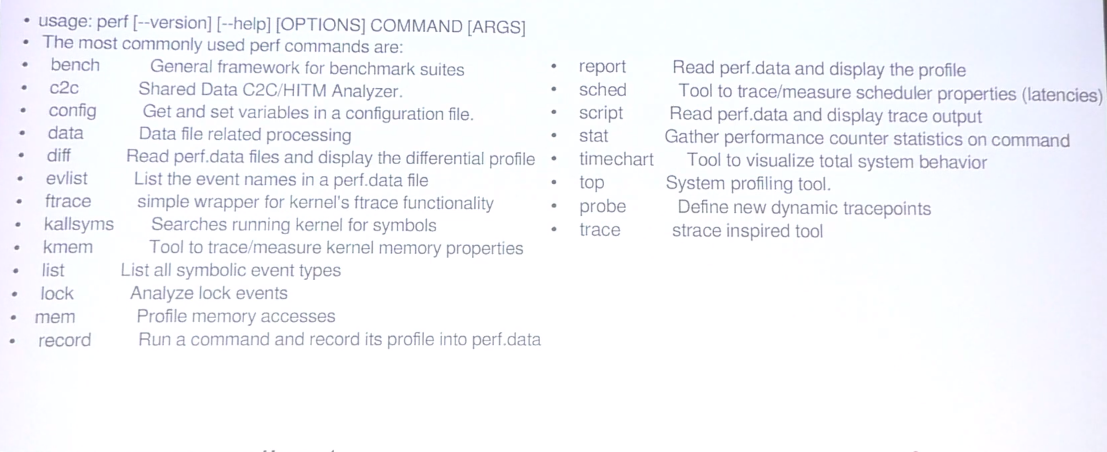
\includegraphics[scale=0.45]{res/perf-base-command.png}
            \caption{Базовые команды в perf}
        \end{center}
    \end{figure}

    Одно из удобных визуальных представлений, что сохраняет профилировщик "--- FlameGraph.

    \begin{figure}[H]
        \begin{center}
            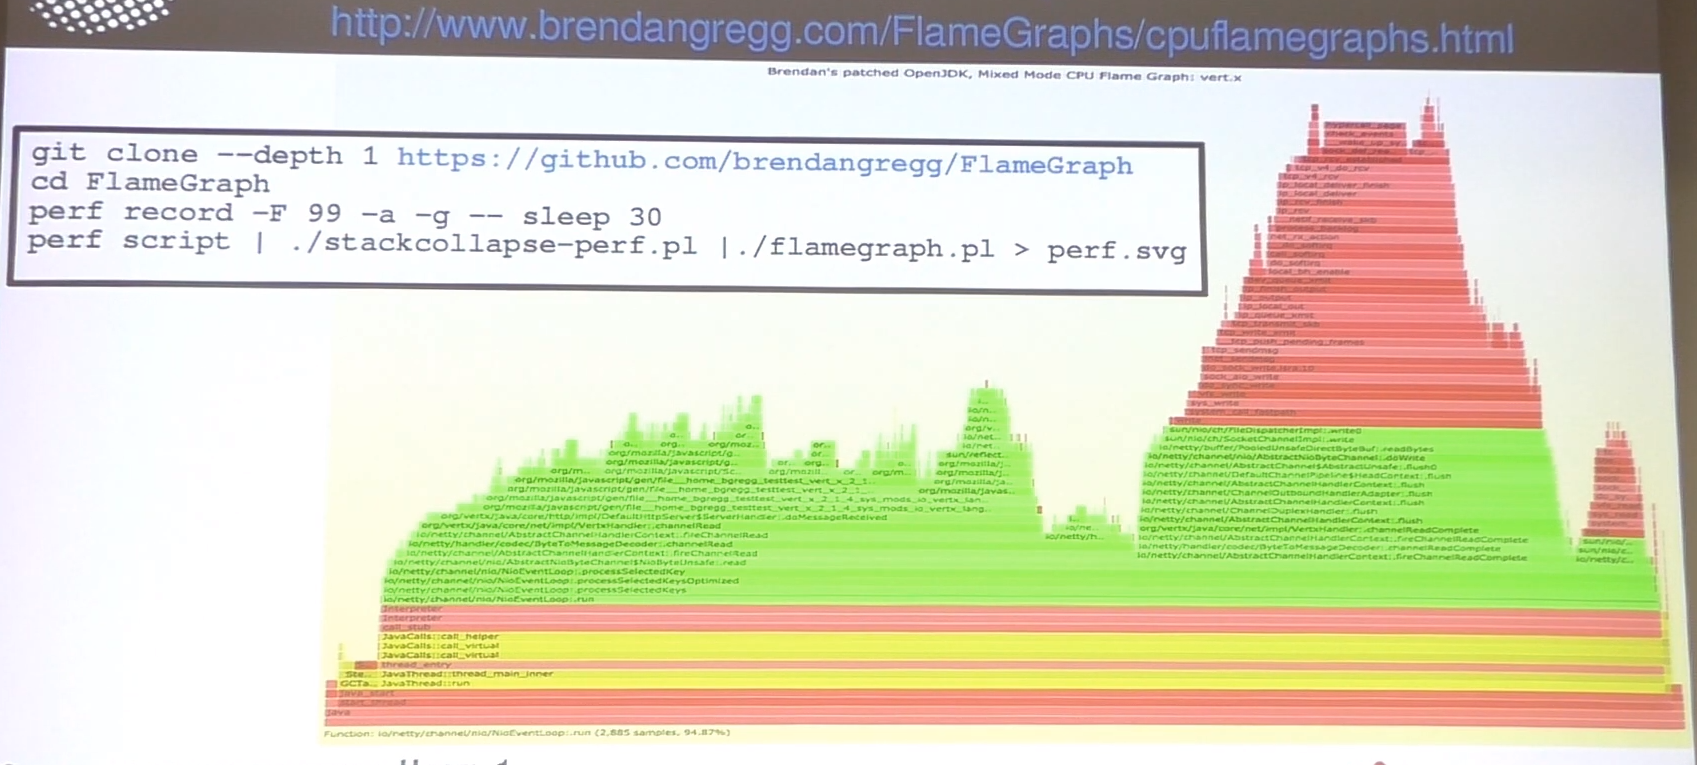
\includegraphics[scale=0.3]{res/FlameGraph.png}
            \caption{FlameGraph}
        \end{center}
    \end{figure}

    \subsection{System tap}

    Еще одно средство сбора информации о подсистеме ядра или пользователя, при этом имеет минимальное воздействие на систему. SystemTap по сути имеет скриптовый синтаксис.

    Основная идея SystemTap состоит в том, чтобы обозначить события и назначить для них обработчики.

    Во время выполнения скрипта, SystemTap занимается мониторингом событий и, как только произойдет событие, ядро системы выполнит обработчик.
    Событиями могут быть начало или конец сессии SystemTap, срабатывание таймера и другие.

    Обработчиком является последовательность скриптовых операторов, которые будут выполнены после срабатывания события. Обычно обработчики извлекают информацию из контекста события или выводят информацию на экран.

    Сессия SystemTap начинается тогда, когда мы выполняем скрипт. В это время происходит следующая последовательность действий:

    \begin{enumerate}
        \item Сначала SystemTap проверяет библиотеку «тапсетов» на наличие использованных в скрипте;
        \item Потом SystemTap транслирует скрипт в Си (язык программирования) и запускает системный компилятор, чтобы создать модуль ядра из скрипта;
        \item SystemTap загружает модуль и активирует все события в скрипте;
        \item Как только происходит событие выполняется обработчик данного события;
        \item Когда все события выполнены, модуль выгружается и сессия завершается;
    \end{enumerate}

    \subsection{Kernel debugger}
    Существует два режима у отладчика ядра: локальный отладчик (предустановлен в системе) и удаленный (предоставляет информацию об системе, находящейся на другом компьютере).

    Чтобы включить компиляцию kdb, вы должны сначала включить kgdb. Параметры компиляции тестов kgdb описаны в главе kgdb test suite 
    
    \href{https://docs.kernel.org/dev-tools/kgdb.html}{https://docs.kernel.org/dev-tools/kgdb.html}.


    Kdb - это упрощенный интерфейс в стиле оболочки, который можно использовать на системной консоли с клавиатурой или последовательной консолью. Вы можете использовать его для проверки памяти, регистров, списков процессов, dmesg и даже установки точек останова для остановки в определенном месте. Kdb не является отладчиком исходного кода, хотя вы можете устанавливать точки останова и выполнять некоторые базовые элементы управления запуском ядра. Kdb в основном предназначена для проведения некоторого анализа, чтобы помочь в разработке или диагностике проблем ядра. 


    \section{Средства для отладки Windows}
    
    \subsection{Встроенные средства}
    
    \textbf{Windows SDK} "--- включает в себя: отладчик, множество утилит, поддерживающих сборку приложений.
    
    \textbf{DTrace on Windows} "--- по сути System tap был скопирован с Dtrance для Windows, тк что по сути у них похожий функционал.

    \textbf{Администрирование} "--- Disk Cleanup, Performance Monitor (очень удобное средство, в котором удобно можно задать параметры), Resource Monitor, Registry Editor Services, System Configuration и тд. (чтобы попасть туда нужно перейти по такому пути: Control Panel -> System and Security -> Administrative Tools).

    \textbf{Task manager} "--- ну, тут не нужно лишних слов.


    Также ссылка на сторонние программы: 
    \href{https://habr.com/ru/company/ua-hosting/blog/280578/}{hhttps://habr.com/ru/company/ua-hosting/blog/280578/}


    \subsection{SysInternals}

    Множество скриптов и программ для управления, диагностики, устранения неполадок и мониторинга всей среды Microsoft Windows. Автор Марк Руссинович, в настоящее время сотрудник Microsoft (Соавтор книги Windows Internals).

    Top SysInternals utils: 

    \begin{itemize}[label=$\bullet$]
        \item PsList and PsKill -- просмотр и остановка процессов (в том числе и удаленно)
        \item Process Explorer - просмотр ресурсов процесса, замена Task Manager
        \item Process Monitor -- просмотр связанных с процессом ресурсов реестра
        \item Autoruns - поиск автозапускаемых программ
        \item Contig - дефрагментирует конкретный файл
        \item PSFile -- позволяет показать открытые файлы, в том числе и удаленно
        \item MoveFile - перемещает заблокированные файлы во время перезагрузки. • Sync - синхронизация файловой системы
        \item TCPview - информация о открытых сетевых соединениях
        \item SDelete - удалить файлы и папки без возможности восстановления
    \end{itemize}

    Тут очень много средств для отлавливания вирусов.

    \subsection{Отладчик ядра WinDbg и KD}
    По умолчанию Windows не загружается в режиме отладчика, для этого есть специальные команды.

    livekd (SysInternals) "--- позволяет перейти в режим отладки без перезагрузки системы.

    Для использования WinDbg необходимо получить символьную информацию (тк в ядре информация хранится в виде 1 и 0, то нужно создать папку для хранения символов переменных, ДЛЯ КАЖДОЙ СБОРКИ ВИНДДЫ НУЖНА СВОЯ СИМВОЛИЧЕСКАЯ ИНФОРМАЦИЯ).

    Пример вызова отладчика:

    \begin{figure}[H]
        \begin{center}
            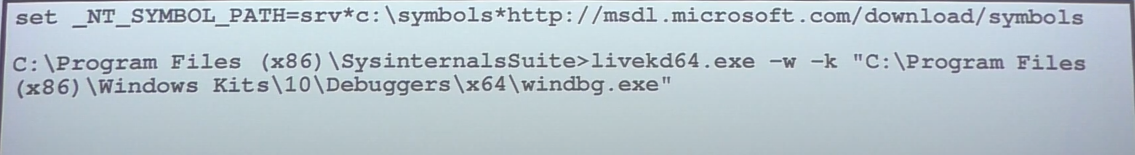
\includegraphics[scale=0.4]{res/example-WinDbg.png}
            \caption{FlameGraph}
        \end{center}
    \end{figure}

    \part{Процессы}

    \section{Основы процессов}

    \subsection{Вычисления}

    По сути наша система компьютерная состоит из ресурсов: процессор, память устройства ввода"=вывода. Приложения, которые мы пишем, решают практическую задачу: Входные данные $\rightarrow$ Обработка $\rightarrow$ Выходные данные. OS по сути находится между оборудованием и приложением. По сути OS представляет абстракции ресурсов и предоставляет их пользователям.


    \subsection{Процесс. Характеристики процесса}
    
    Каждая из подсистем рассматривает процесс в своем ключе.
    
    \hfill \break
    И так, повторим, процесс это: 

    \begin{itemize}[label=$\bullet$]
        \item Выполняемая программа;
        \item Экземпляр программы, выполняющийся на компьютере;
        \item Сущность, которая может быть назначена процессору и выполнена на нем;
        \item Единица активности, характеризуемая выполнением последовательных команд, текущим состоянием и связанным с ней множеством системных ресурсов;
    \end{itemize}

    \hfill \break
    Характеристики процесса в момент времени:

    \begin{itemize}[label=$\bullet$]
        \item Уникальный идентификатор;
        \item Состояние (выполнение, очередь, ожидание);
        \item Приоритет по отношению к другим процессам;
        \item Счетчик команд;
        \item Указатели на область памяти процесса;
        \item Контекст процесса (регистры, user / kernel);
        \item Статус ввода"=вывода;
        \item Счетчики системных ресурсов;
        \item Права доступа процесса;
        \item и тд; 
    \end{itemize}
    
    \subsection{Состояние процессов и разделение ресурсов}

    Рассмотрим ситуацию, где есть два процесса с одинаковым приоритетом и числом доступных ресурсов. Вспомним, что в таком случае у нас для этих процессов будет выделено одинаковое количество процессорного времени.

    \begin{figure}[H]
        \begin{center}
            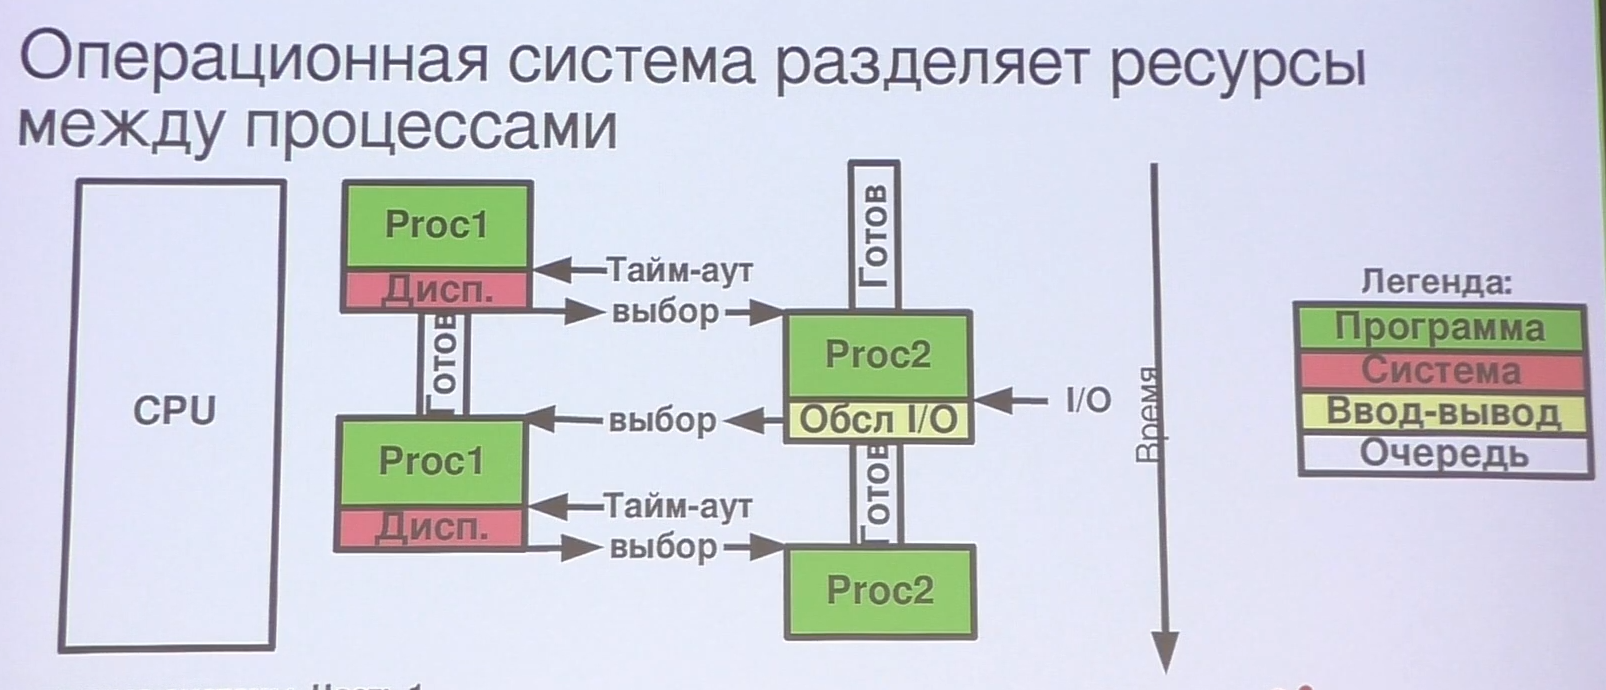
\includegraphics[scale=0.3]{res/example-two-process.png}
            \caption{}
        \end{center}
    \end{figure}

    Как происходит распределение ресурсов процессора между процессами? 
    
    \begin{definition}
        \textbf{Квант} "--- единица времени, периодичность, с которой система проверяет, не выполняется ли процесс слишком долго.
    \end{definition}

    Раз в квант система проверяет, закончилось ли процессорное время у процесса, если да, то диспетчер берет другой, а этот снова кладет в очередь.
     
    Это все делается для того, чтобы примерно одинаковые процессы выполнялись одинаковое количество времени.

    \textbf{Рассмотрим состояния процесса}

    \begin{figure}[H]
        \begin{center}
            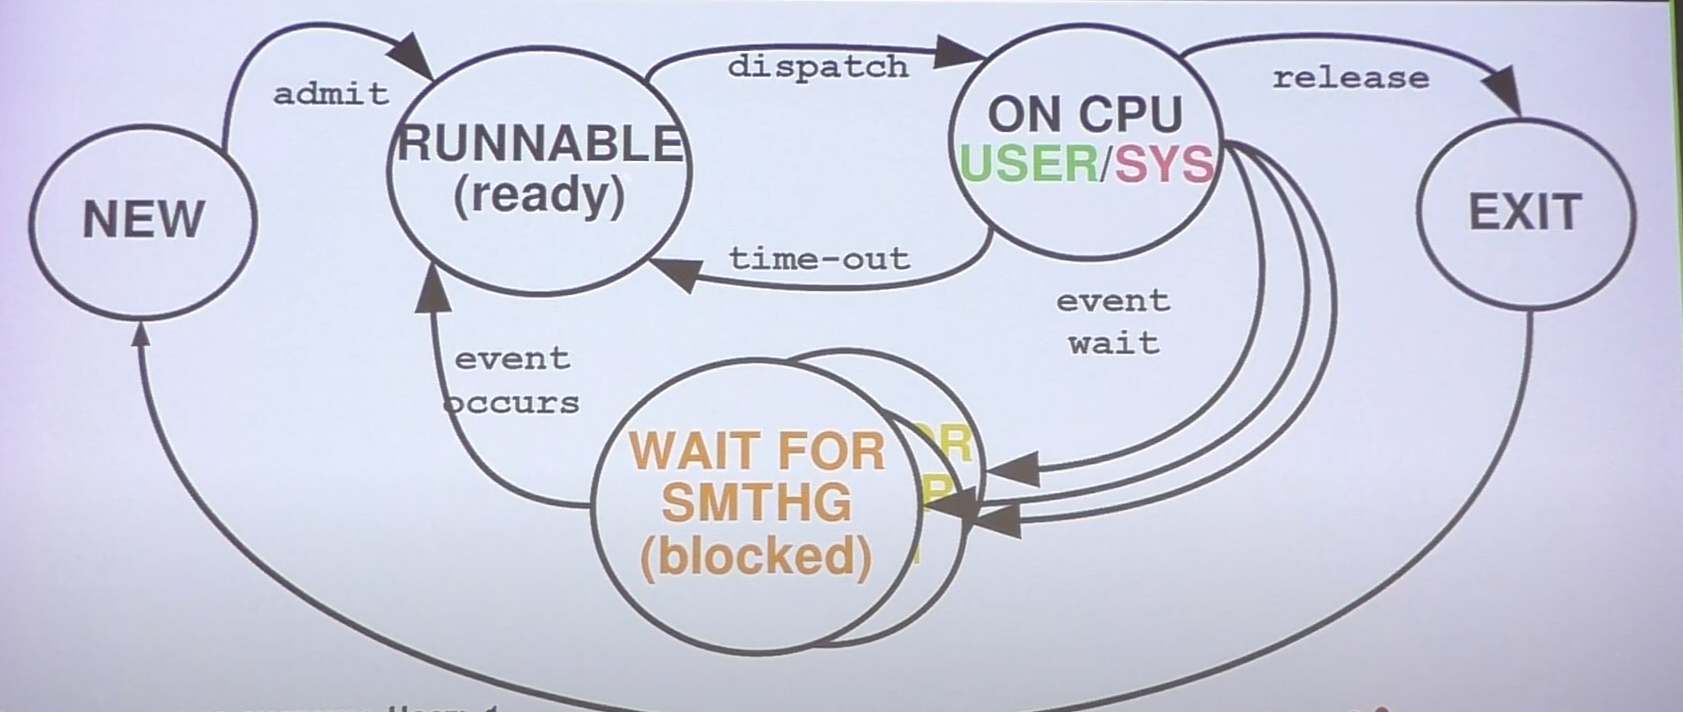
\includegraphics[scale=0.3]{res/model-of-process-with-5-states.png}
            \caption{Цикл работы процесса}
        \end{center}
    \end{figure}

    \begin{itemize}[label=$\bullet$]
        \item Ready "--- готов к выполнению, это значит процессор может взять этот процессор на исполнение. Есть все необходимые ресурсы, которые позволяют ему выполнится. К примеру, страницы памяти, сигнал завершения ввода вывода;
        \item On CPU "--- если процессор свободен, то мы можем назначить на него процесс. Процесс может работать в двух режимах user и sys. Во время выполнения процесса эти режимы могут переключаться;
        \item Выход из состояния On CPU в двух случаях "--- процесс выполнен или у него закончилось системное время;
    \end{itemize}

    \hfill \break
    \textbf{New state} "--- процесс создан, но еще не размещен в очереди процессов, готов к исполнению. 

    \hfill \break
    \textbf{Exit state} "--- процесс не может продолжить выполнение. (Структуры процесса еще существуют).

    Причины попадания в состояние:
    
    \begin{itemize}[label=$\bullet$]
        \item Нормальное завершение (вызов exit);
        \item превышение лимитов на время выполнения;
        \item Недостаток памяти;
        \item Ошибки границ и защиты памяти;
        \item Арифметическая ошибка;
        \item Ошибка ввода-вывода;
        \item Неправильная или привилегированная инструкция;
        \item Команда оператора или OS;
        \item Завершение или запрос родительского процесса;
    \end{itemize}

    \hfill \break
    \textbf{Runnable state} "--- процесс обладает всеми ресурсами для выполнения, но нет возможности исполниться.

    Причины попадания в состояние:

    \begin{itemize}[label=$\bullet$]
        \item Низкий приоритет по сравнению с другими процессами;
        \item Ожидания освобождения CPU;
        \item Закончился квант времени;
    \end{itemize}

    \hfill \break
    \textbf{Runnable state} "--- процесс выполняется на процессоре.

    Процесс остается в этом состояние если:

    \begin{itemize}[label=$\bullet$]
        \item не истек квант времени;
        \item Ожидание на спин"=блокировке;
        \item В Runnable состоянии нет процессов с более высоким приоритетом;
        \item Обслуживание высокоприоритетных прерываний;
        \item Нет блокирующих вызовов (ввод вывод, ожидание блокировки);
    \end{itemize}


    \hfill \break
    \textbf{Wait (blocked) state} "--- ожидания событий OS, освобождения блокировки. Процесс не расходует ресурсов CPU, процесс может находиться в ожидании неопределенно долго. Бывает процесс не убивается, пока он не будет разблокирован (самое простое, перезагрузить OS).

    Состояние продолжается пока:

    \begin{itemize}[label=$\bullet$]
        \item освободится блокировка;
        \item Придет сообщение OS о наступление ожидаемого события.
    \end{itemize}

    \section{Пейджинг и свопинг}
    
    \subsection{Paging Swapping}

    Как правило, основной памяти всегда мало, если появляется свободная память программисты сразу пытаются ее заполнить. А также в системе обычно большое количество запущенных процессов. 

    Давайте поместим блокируемый процесс на диск и освободим основную память для других процессов.

    \begin{definition}
        \textbf{Paging} "--- выгрузка или загрузка неиспользуемых страниц процесса на диск.
    \end{definition}

    \begin{definition}
        \textbf{Swapping} "--- выгрузка всего процесса, кроме критически важных для ядра структур.
    \end{definition}

    \begin{figure}[H]
        \begin{center}
            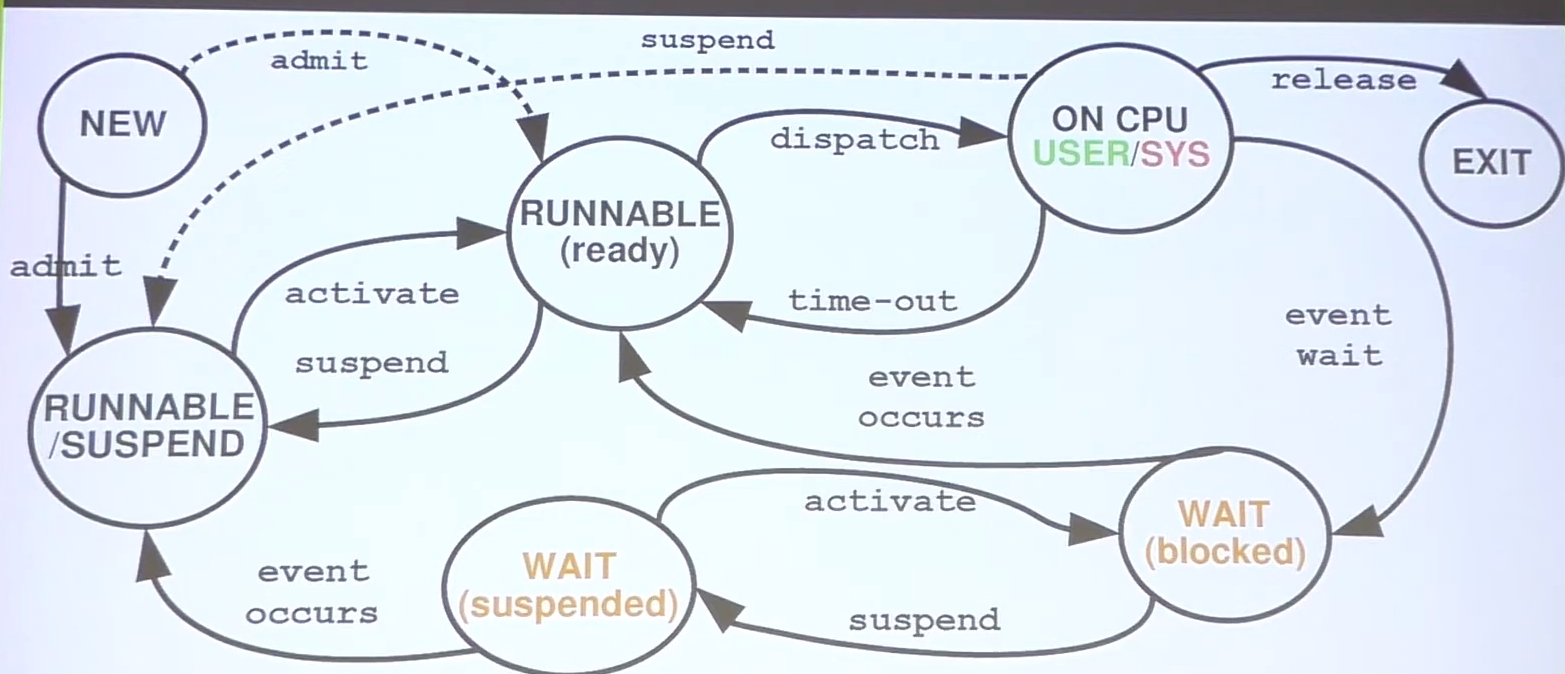
\includegraphics[scale=0.3]{res/model-of-process-with-7-states.png}
            \caption{Модель цикла процесса с 7 состояниями}
        \end{center}
    \end{figure}

    На картинке можно наблюдать цикл состояния процесса с Pagin / Swapping. 

    Изменения в том, что мы разделили состояние Wait и Runnable на две части.

    Почему стрелочка из New идет в Runnable Suspend? Тк процесс создается долго, в современных системах, создается минимальный костяк процесса, без мепинга, и отправляется в приостановленное состояние, чтобы можно было быстро отчитаться о создание процесса.
    
    Также интересное замечание, что может создаться такая ситуация, что при большом количестве процессов, может выстроиться очередь на блокировку процессов, тогда вся система начнет глобально тормозить.

    \subsection{Дополнительные состояния процессора}
   
    \hfill \break
    \textbf{Wain / Suspend state} "--- процесс приостановлен и выгружен в область подкачки. По событию Suspend процесс выгружается на диск. По событию Active загружается в основную память. (Данные действия повышают нагрузку на дисковую подсистему).

    Причины попадания в состояние:

    \begin{itemize}[label=$\bullet$]
        \item Длительное ожидание события операционной системы;
        \item Недостаток памяти (зачем держать в памяти процесс, который не имеет возможности исполниться).
    \end{itemize}

    \hfill \break
    \textbf{Runnable / Suspend state} "--- процесс готов к выполнению, но выгружен из памяти.

    Причины:

    \begin{itemize}[label=$\bullet$]
        \item Был неготов, выгружен, но произошло событие, которое позволяет выполниться;
        \item Desperate memory conditions;
        \item Команда пользователя;
        \item Создание процесса в минимальном варианте, без, к примеру создания сегментов памяти.
    \end{itemize}

    \section{Управление процессами}

    \subsection{Управляющие таблицы}
    
    \begin{figure}[H]
        \begin{center}
            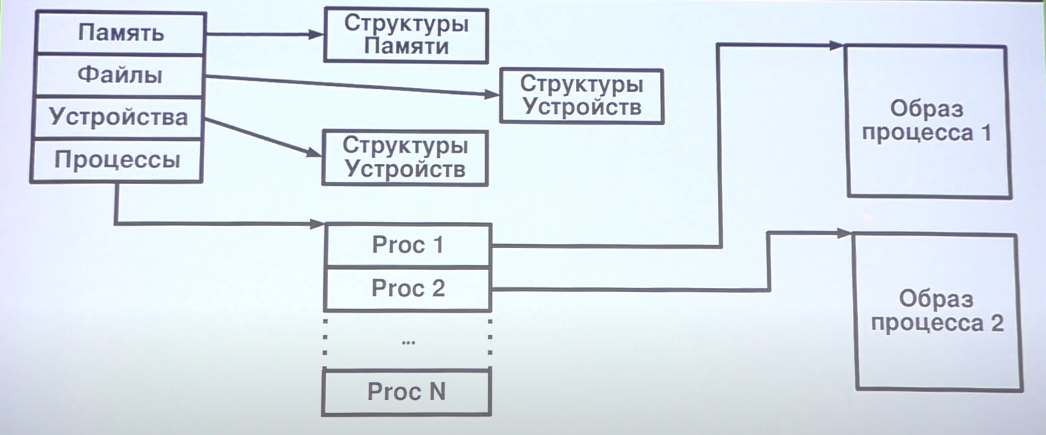
\includegraphics[scale=0.4]{res/general-structure-of-control-table.png}
            \caption{Общая структура управляющей таблицы}
        \end{center}
    \end{figure}

    \subsection{Образ процесса}

    Допустим у нас есть код написанный на языке C.

    \begin{minted}[fontsize=\footnotesize]{cpp}
        #include <stdio.h>

        int var_int_data[1024]; static char var_char_data[4096];
        
        void foo(int var_inc) {
            int var_a = 10;
            static int var_sa = 10;
            
            var_a += var_inc;
            var sa += var inc; printf("a = %d, sa = %d\n", var_a, var_sa);
        }
        int main(int arge, char**argv) { 
            int var_i;
            
            for (var_i = 0; var_i < 10; ++var_i) 
                foo (var_i);
        }
    \end{minted}

    Давайте попробуем понять, где что находится?
    
    \begin{figure}[H]
        \begin{center}
            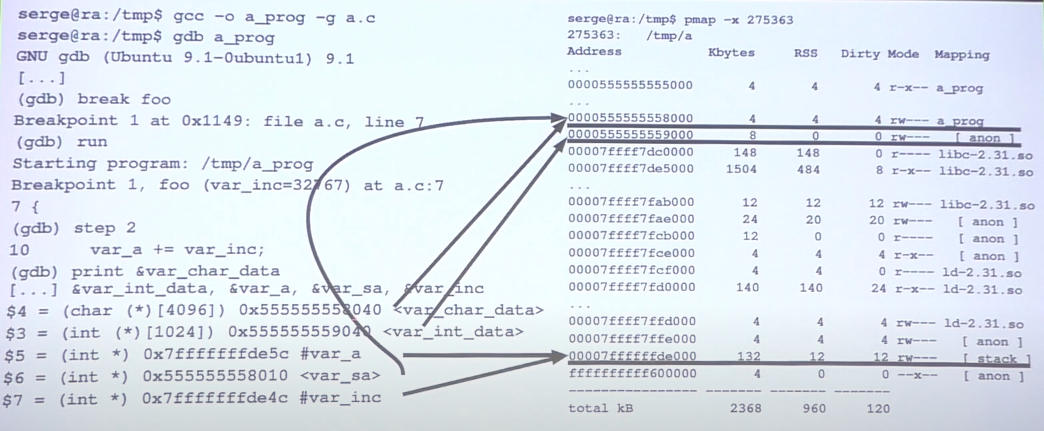
\includegraphics[scale=0.5]{res/example-C-programm-for-process.png}
            \caption{}
        \end{center}
    \end{figure}

    Запомним: rw "--- сегмент данных или куча (anon), а также у нас снизу есть еще и стек. Строки где одни -------, значат, что к этим страницам обратиться нельзя.

    Пройдемся дебагером, и увидим что массив чаров у нас ушел в сегмент данных, по адресу ....8040. А массив интов, ушел в кучу по адресу ....9040. Важно помнить, что разные компиляторы ведут себя по разному. Также мы видим, статические переменные попали в стек. 
    
    \begin{figure}[H]
        \begin{center}
            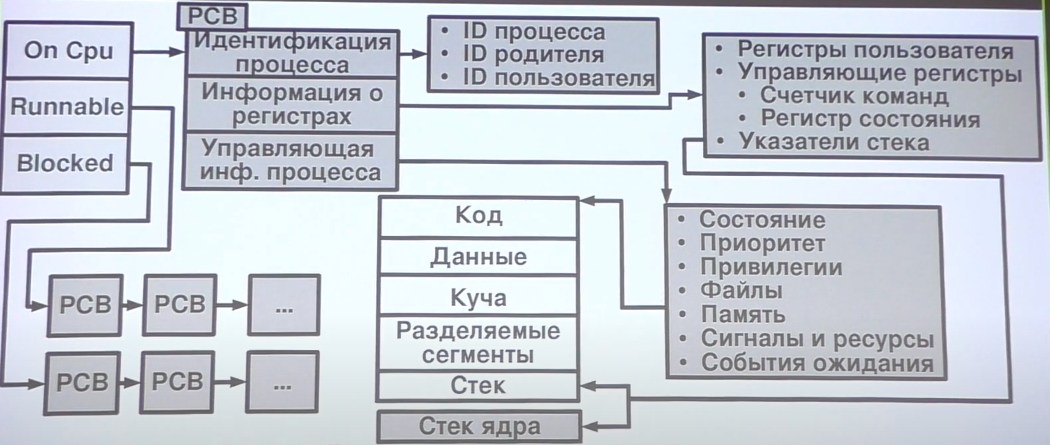
\includegraphics[scale=0.45]{res/Process-Control-Block.png}
            \caption{Управляющий блок процесса}
        \end{center}
    \end{figure}

    В управляющем блоке процесса содержится информация о: инициализации процесса,какие регистры ему принадлежат, а также многое другое)).

    Если смотреть на наш процесс внутри операционной системы, то есть несколько очередей, в которых содержатся ссылки на управляющие блоки процессов. Все эти структуры тесно связаны между собой, иногда переходят из одной очереди в другую.

    \subsection{Функции OS}

    Функции OS связанные с процессами:

    \hfill \break
    \textbf{Управление процессами}
    \begin{itemize}[label=$\bullet$]
        \item Создание и завершение процессов;
        \item Планирование и диспетчеризация процессов;
        \item Переключение процессов;
        \item Синхронизация и поддержка обмена информацией между процессами;
        \item Организация управляющих блоков процессов
    \end{itemize}

    \hfill \break
    \textbf{Управление вводом"=выводом}
    \begin{itemize}[label=$\bullet$]
        \item Управление буферами;
        \item Выделение процессам каналов и устройств ввода "= вывода
    \end{itemize}

    \hfill \break
    \textbf{Управление памятью}
    \begin{itemize}[label=$\bullet$]
        \item Выделение адресного пространства процессам;
        \item Управление страницами и сегментами;
        \item Пейджинг и Свопинг;
    \end{itemize}

    \hfill \break
    \textbf{Функции поддержки}
    \begin{itemize}[label=$\bullet$]
        \item Обработка прерываний;
        \item Учет пользования ресурсами;
        \item Текущий контроль системы;
    \end{itemize}


    \hfill \break
    \textbf{Вспомним, что} создание процесса включает в себя:

    \begin{itemize}[label=$\bullet$]
        \item Присвоение уникального идентификатора;
        \item Выделение памяти;
        \item Инициализация PCB;
        \item Постановка процесса в очередь ядра;
        \item Создание потоков ввода"=вывода;
        \item Создание других управляющих структур данных.
    \end{itemize}

    \subsection{Процессы SVR4}

    На картинке представлен цикл создания процесса в UNIX. 

    \begin{figure}[H]
        \begin{center}
            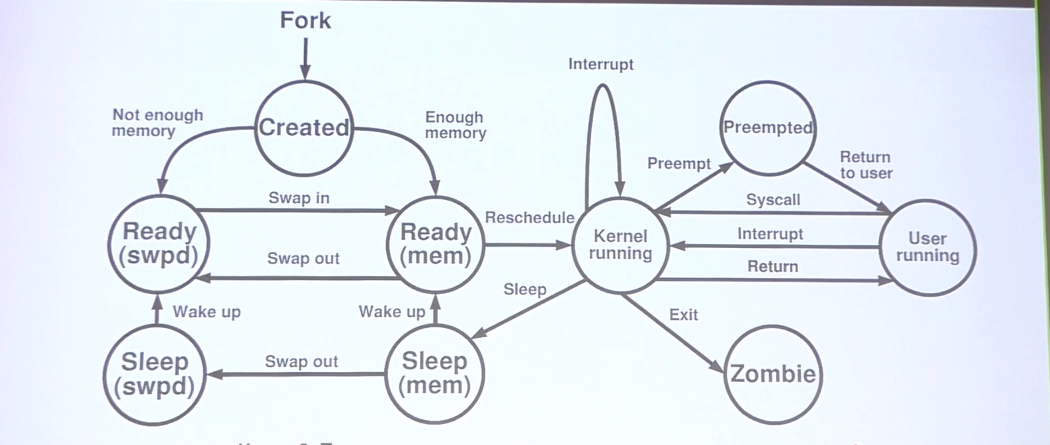
\includegraphics[scale=0.45]{res/SVR4.png}
            \caption{Создание процессов в UNIX}
        \end{center}
    \end{figure}

    Можем наблюдать явно использование процесса в user и kernel режимах.

    \section{Потоки}

    \subsection{Понятие потока}

    Абстрактная модель процесса подразумевает владение ресурсами, а также планирование и диспетчеризацию. 

    По сути, процесс является единицей группировки ресурсов, а Tread "--- единица выполнения программного кода.

    Tread содержит: Состояние выполнения, Сохранение контекста потока, Стек, Локальные переменные, Доступ к памяти и ресурсам процесса владельца.

    \subsection{Связь потоков и процессов}

    \begin{figure}[H]
        \begin{center}
            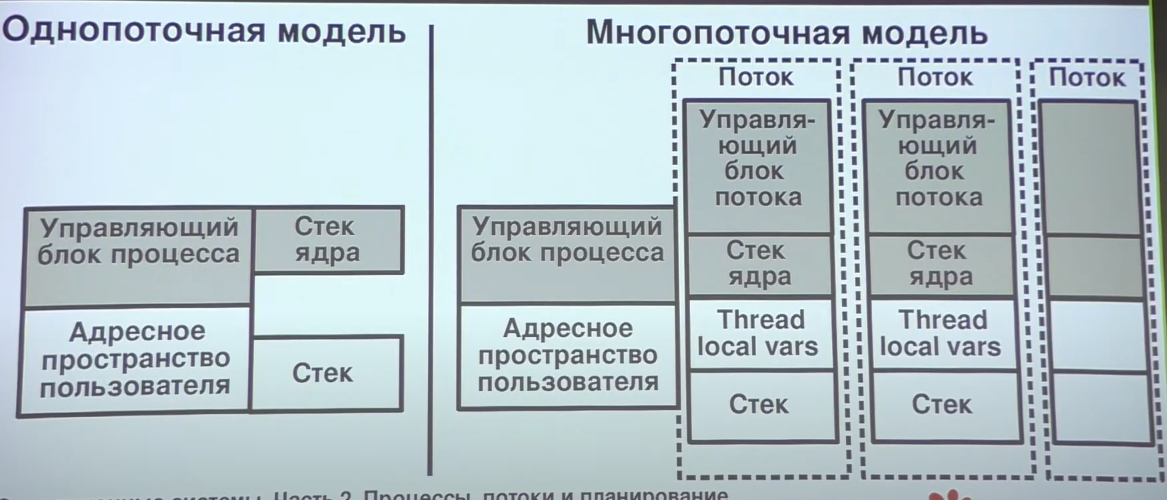
\includegraphics[scale=0.40]{res/connection-of-kernel-and-thread-structures.png}
            \caption{Связь структур ядра и потока}
        \end{center}
    \end{figure}

    Как мы видим у нас также есть управляющий блок процесса. Важно заметить, что структуры отвечающие за управления у потоков разные, а ресурсы одни.

    Главное преимущество потоков в быстродействие, все действия для них выполняются быстрее (Переключение между потоками быстрее, тк переключается только контекст, убиваются они тоже быстрее, но лучше лишний раз не убивать, тк это все равно энергозатратно). Даже в однопоточных моделях есть преимущества (работа в приоритетном и фоновом режиме, асинхронная работа частей программы, модульная структура программы). 

    \subsection{Состояния потока}

    \begin{figure}[H]
        \begin{center}
            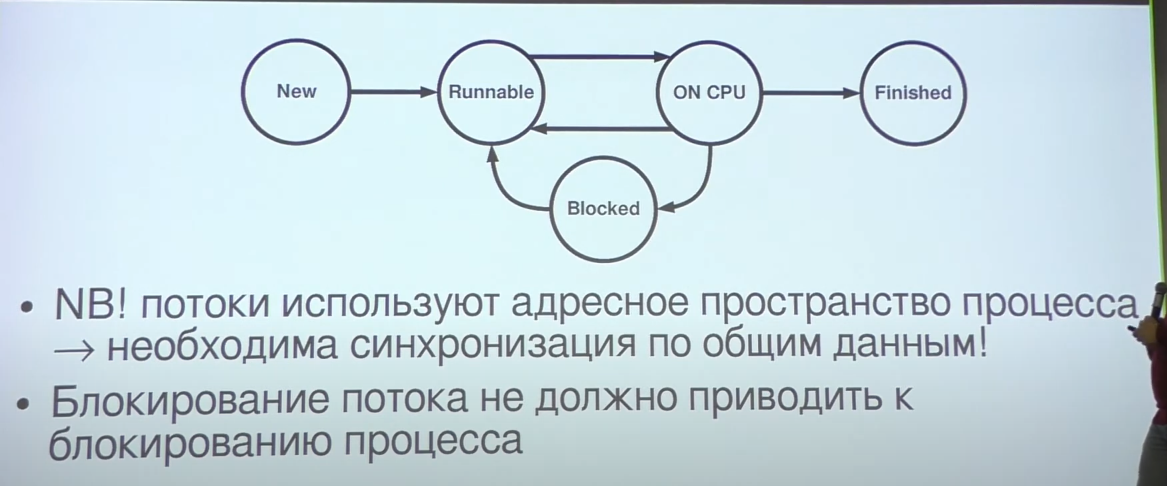
\includegraphics[scale=0.40]{res/state-of-tread.png}
            \caption{Состояние потоков}
        \end{center}
    \end{figure}

    Как мы видим, состояния потоков не сильно отличаются от состояний процессов, за исключением того, что нет структур отвечающих за диспетчеризацию.

    \subsection{Варианты реализации}

    User level Tread "--- реализуется библиотеками или приложениями на стороне пользователя.

    Kernel level Tread "--- реализуется ядром. 

    Основная разница заключается в том, что для User lvl для переключения между потоками не нужно уходить в ядро.

    В данный момент чаще всего используется модель KLT, сколько потоков мы породили на уровне пользователя, столько получим и на уровне ядра.

    \begin{figure}[H]
        \begin{center}
            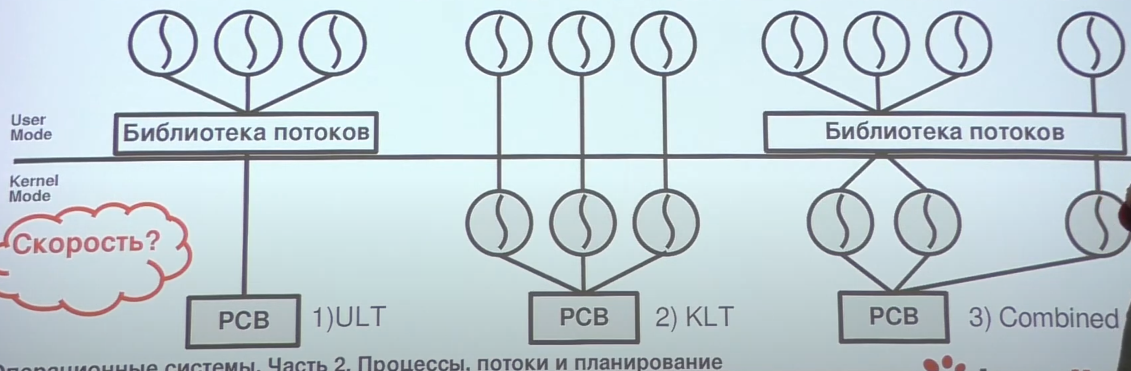
\includegraphics[scale=0.40]{res/models-of-tread.png}
            \caption{Модели потоков}
        \end{center}
    \end{figure}


    \subsection{Закон Амдала}

    На сколько можно ускорить программу на N процессах с использованием потоков?

    \begin{theorem}
        \textbf{Закон Амдала} "--- ускорение = время работы на одном процессоре / время работы на N процессах.
    \end{theorem}

    \huge
    ускорение =  $\frac{T * (1 - f) + T * f}{T * (1 - f) + \frac{T * f}{N}} = \frac{1}{(1-f) + \frac{f}{N}}$
    \normalsize

    \hfill \break
    Где T "--- время работы, f "--- доля распараллеливания [0,1). Когда f мало, использование параллельного выполнения неэффективно. Когда N стремится к бесконечности, то ускорение ограничено $\frac{1}{1 - f}$.

    \begin{figure}[H]
        \begin{center}
            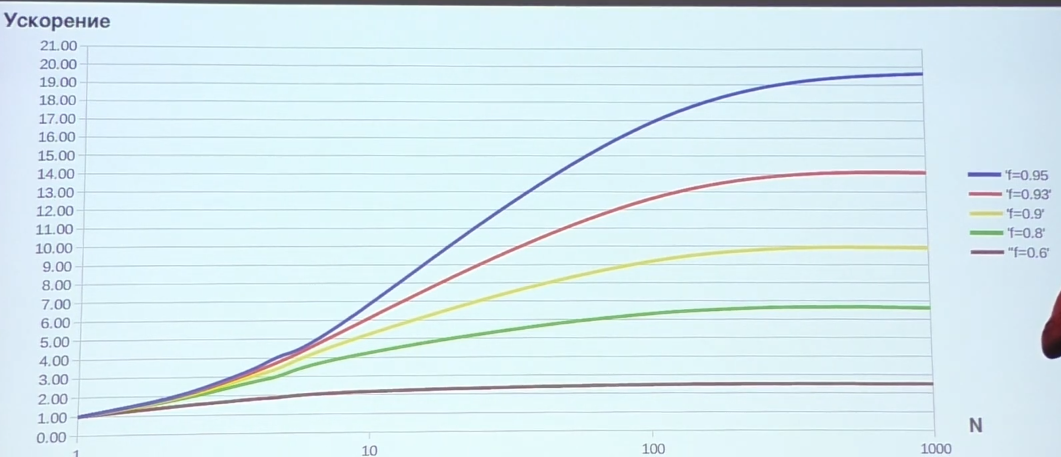
\includegraphics[scale=0.40]{res/Amdahl's-law.png}
            \caption{Визуализация закона Амдала}
        \end{center}
    \end{figure}

    \section{Параллельные вычисления. Блокировки}

    \subsection{Параллельность программ}
    
    \begin{figure}[H]
        \begin{center}
            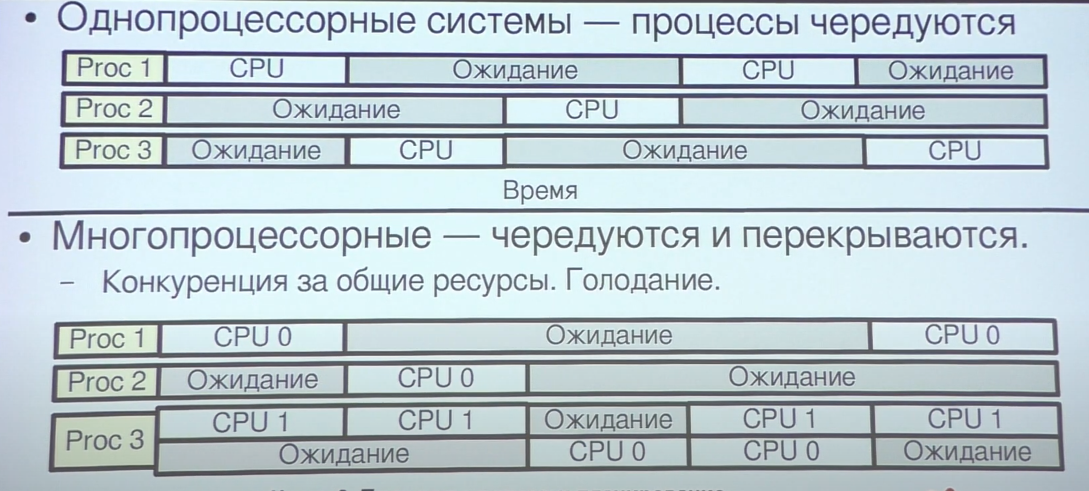
\includegraphics[scale=0.40]{res/Parallel-Computing-Mechanism.png}
            \caption{Механизм параллельных вычислений}
        \end{center}
    \end{figure}

    Голодание часто втречается в ситуации, где блокировкой процесса A владеет низкоприорететный процесс B. В следствие этого, процесс B отодвигают процессы с более высоким приорететом, из"=за этого процесс А не может выполниться.


    \subsection{Функции OS поддержки параллельности}
    Требуемые функции OS:

    \begin{itemize}[label=$\bullet$]
        \item Отслеживание русурсов процесса или потока;
        \item Распределение и освобождение ресурсов для процесса или потока;
        \item Защита ресурсов процесса или потока от непреднамеренного воздействия на них других процессов или потоков;
        \item Независимость результата процесса или потока, от скорости его выполнения;
    \end{itemize}

    \subsection{Проблемы}

    \begin{itemize}[label=$\bullet$]
        \item Взаимоисключения (Mutual Exclusion) "--- процессы или потоки не должны одновременно использовать критический ресурс.
        \item Взаимоблокировки (Dead Lock) "--- процессы или потоки не должны взаимозахватывать требуемые ресурсы;
        \item Голодание (Starvation) "--- конкуренция за ресурсы не должна порождать невозможность доступа к ресурсу;
    \end{itemize}

    
    \subsection{Функции OS поддержки параллельности}

    \textbf{Требования OS к взаимным исключениям}
    \begin{itemize}[label=$\bullet$]
        \item Взаимные исключения осуществляются в принудительном порядке (в критическом участке только один процесс / поток);
        \item Процесс / поток не должен влиять на другие процессы / потоки в некритическом участке;
        \item Противодействие бесконечному ожиданию доступа к критическому участку;
        \item Вход в свободный критический участок должен незамедлительно предоставляться;
        \item Отстуствие предположений о количестве процессов и их скорости;
        \item Ограничение времени нахождения в критическом участке;
    \end{itemize}

    Аппаратной поддержкой взаимных исключений являются атомарные инструкции: TAS, CAS, CMPXCHG и тд.

    \subsection{Взаимодействие процессов / потоков}

    Процессы / потоки могут не знать ничего друг о друге, тогда происходит конкуренция за ресурсы, взаимоисключения, взаимоблокировки, голодание.

    Процессы / потоки сотрудничают используя общий ресурс, это может вызвать: взаимоисключения, взаимоблокировки, голодание, связь данных.

    Процессы / потоки совместимо выполняются, это может вызвать: взаимоблокировки, голодание.


    \section{Примитивы синхронизации OS}

    \subsection{Семафоры, мьютексы}

    \begin{definition}
        \textbf{Семафоры} "--- захват и освобождение множественного ресурса.
    \end{definition}

    \begin{figure}[H]
        \begin{center}
            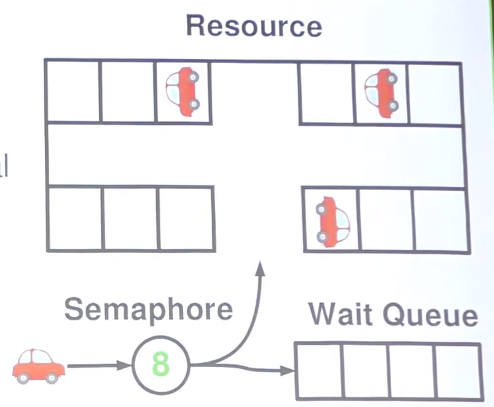
\includegraphics[scale=0.40]{res/example-Semaphore.png}
            \caption{Пример работы семафора}
        \end{center}
    \end{figure}


    \begin{definition}
        \textbf{Мьютексы} "--- блокировка или освобождение ресурса единственным процессом или потоком (создание критических секций). Существует большое количество мьютексов: блокирующие, спин, адаптивные и тд.
    \end{definition}

    \begin{figure}[H]
        \begin{center}
            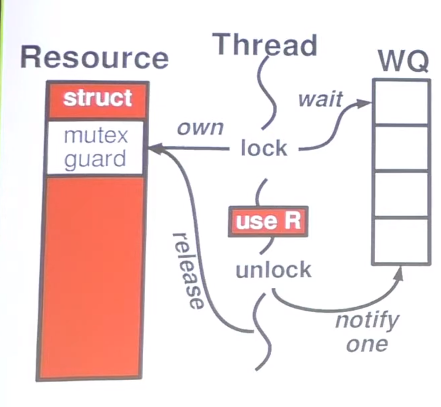
\includegraphics[scale=0.40]{res/example-Mutex.png}
            \caption{Пример работы мьютекса}
        \end{center}
    \end{figure}


    Для каждого мьютекса или семафора очередь ожидания своя.

    Важно помнить, что захват мьютекса должен быть как можно короче, желательно не больше пары строчек кода.

    Если сообщение о разблокировке мьютекса приходит не от того потока, который заблокировал его, то выводится сообщение об ошибке.

    Частое решение проблеммы Priority Inversion, когда у нас поток с высоким приоретом не может выполниться, тк мьютекс заблокирован потоком, который также не может пройти дальше из"=за низкого приоретета "--- это наследование приоретета до разблокировки критической секции.

    \begin{definition}
        \textbf{Условные переменные} "--- примитив синхронизации, обеспечивающий блокирование одного или нескольких потоков до момента поступления сигнала от другого потока о выполнении некоторого условия или до истечения максимального промежутка времени ожидания. Условные переменные используются вместе с ассоциированным мьютексом и являются элементом некоторых видов мониторов.
    \end{definition}

    У условных переменных есть 3 состояния: wait, signal, broadcast

    \textbf{Producer / Consumer Problem} "--- проблема загрузки в буфер, когда из него при этом происходит чтение. Для этого существуют два индекса, которые все контролируют.

    \begin{figure}[H]
        \begin{center}
            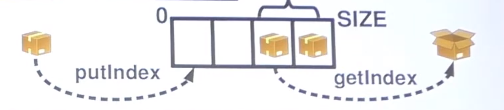
\includegraphics[scale=0.60]{res/Producer-Consumer-Problem.png}
            \caption{ПProducer / Consumer Problem }
        \end{center}
    \end{figure}
    
    \begin{definition}
        \textbf{Мониторы} "--- конструкции высокоуровневых языков программирования, которые скрывают низкоуровневые примитивы синхронизации.
    \end{definition}

    \begin{definition}
        \textbf{Флаги событий} "--- блокировка секций путем проверки условий на флагах. Похожая реализация у event в python.
    \end{definition}

    \textbf{Multiple reader, single writer locks} "--- когда читатели читают, они захватывают read lock, количество одновременных читателей содержится в rwlock. Когда писателю нужно записать, он устанавливает требование записи (want write) и ожидает на rwlock, который ждет освобождения readlock.
 

    \begin{definition}
        \textbf{Message passing} "--- является одной из популярных концепций параллельного программирования. Она часто используется при создании сложных распределенных систем с высокой степенью параллелизма. Реализация этой концепции представлена в языках программирования в качестве актёров (actor) или агентов (agent).
    \end{definition}

    \begin{itemize}[label=$\bullet$]
        \item Решение состоит из изолированных компонент, которые работают параллельно (в параллельных потоках из пула потоков). Взаимодействие между компонентами идет через обмен сообщениями по определенному протоколу. Сетевые компоненты могут использовать TCP, UDP, HTTP, и т.д. Локальные взаимодействуют через протокол, определенный конкретный языком его реализации или библиотекой.
        \item Компонент определяет логику обработки входных сообщений. Последние попадают в очередь (queue) и последовательно достаются из нее для обработки.
        \item Компонент может быть владельцем некоторых ресурсов и быть их провайдером для других компонент. Ресурсом могут быть: данные в определенном формате в оперативной памяти, аппаратно-программный ресурс или их комбинация.
        \item Компонент имеет определенное состояние, которое может инкапсулировать ресурс (из предыдущего пункта), или, как в случае машины состояний (state machine), может быть выражен в виде определенного алгоритма обработки сообщений, который переводит его в другое состояние.
        \item Интерфейс между компонентами:
            \begin{itemize}
                \item postSync, postAsync "--- послать сообщение компоненте синхронно или асинхронно.
                \item receiveSync, receiveAsync "--- получить сообщение от компонента синхронно или асинхронно. Асинхронное ожидание состоит в том, что поток как ресурс возвращается системе и может быть использован для другой работы. В этом случае система регистрирует функцию обратного вызова (callback) на определенное событие.
                \item tryReceive функции "--- аналогичные вышеперечисленным, но имеющим определенную задержку для получения данных.
            \end{itemize}
        \item Концепция тесно связана с понятием асинхронного исполнения.
    \end{itemize}

    \section{Процессы и потоки в Linux}
    \section{Примитивы синхронизации в Linux}
    \section{Процессы и потоки в Windows}
    \section{Примитивы синхронизации в Windows}

    \section{Полезные утилиты}

    Linux kernel map "--- \href{https://makelinux.github.io/kernel/map/}{https://makelinux.github.io/kernel/map/}

    Сайт с рекомендациями  по отладке Linux "--- 
    
    \href{https://brendangregg.com/linuxperf.html}{https://brendangregg.com/linuxperf.html}


\end{document}